\documentclass[specification,annotation,times]{itmo-student-thesis}
% 

%% Опции пакета:
%% - specification - если есть, генерируется задание, иначе не генерируется
%% - annotation - если есть, генерируется аннотация, иначе не генерируется
%% - times - делает все шрифтом Times New Roman, собирается с помощью xelatex
%% - languages={...} - устанавливает перечень используемых языков. По умолчанию это {english,russian}.
%%                     Последний из языков определяет текст основного документа.

%% Делает запятую в формулах более интеллектуальной, например:
%% $1,5x$ будет читаться как полтора икса, а не один запятая пять иксов.
%% Однако если написать $1, 5x$, то все будет как прежде.
\usepackage{icomma}

%% Один из пакетов, позволяющий делать таблицы на всю ширину текста.
\usepackage{tabularx}

\usepackage{courier}

\usepackage{svg}

\hyphenation{Лидер/Последователи}
\hyphenation{Полусинхронный/Полуреактивный}

%% Данные пакеты необязательны к использованию в бакалаврских/магистерских
%% Они нужны для иллюстративных целей
%% Начало
\usepackage{tikz}

\usetikzlibrary{arrows}
\usetikzlibrary{positioning}

%% Указываем файл с библиографией.
\addbibresource{master-thesis.bib}

\begin{document}

\studygroup{P42111}
\title{Разработка и реализация методов эффективного взаимодействия процессов в распределенных системах}
\author{Губарев Владимир Юрьевич}{Губарев В.Ю.}
\supervisor{Косяков Михаил Сергеевич}{Косяков М.С.}{к.т.н.}{доцент ФПИиКТ}
\publishyear{2020}
%% Дата выдачи задания. Можно не указывать, тогда надо будет заполнить от руки.
%\startdate{01}{сентября}{2017}
%% Срок сдачи студентом работы. Можно не указывать, тогда надо будет заполнить от руки.
%\finishdate{31}{мая}{2019}
%% Дата защиты. Можно не указывать, тогда надо будет заполнить от руки.
%\defencedate{15}{июня}{2019}
%
%\addconsultant{Белашенков Н.Р.}{канд. физ.-мат. наук, без звания}
%\addconsultant{Беззубик В.В.}{без степени, без звания}

\secretary{Болдырева Е.А.}

\specialty{09.04.04 ''Программная инженерия``}
\specialization{''Информационно-вычислительные системы``}

\faculty{ПИиКТ}

\programhead{Бессмертный И.А.}{доцент, д.т.н.}

%% Задание
%%% Техническое задание и исходные данные к работе
\technicalspec{Требуется разработать и реализовать эффективные методы межпроцессного взаимодействия в пределах одного физического узла. Межпроцессное взаимодействие как с локальными, так и с удаленными процессами должно осуществляться через единый программный интерфейс. Интерфейс должен автоматически выбирать наиболее эффективный метод межпроцессного взаимодействия и скрывать реализацию от пользователя.}

%%% Содержание выпускной квалификационной работы (перечень подлежащих разработке вопросов)
\plannedcontents{
\begin{enumerate}
\item Обзор предметной области и постановка цели работы.
\item Разработка и реализация методов эффективного взаимодействия процессов.
\item Экспериментальное исследование и обработка результатов.
\end{enumerate}}

%%% Исходные материалы и пособия 
\plannedsources{\begin{enumerate}
\item Косяков М.С. Введение в распределенные вычисления. Учебное пособие / М.С. Косяков. --	СПб: СПбГУ ИТМО, 2014. -- 155 с.
\item Schmidt D.C. et al. Pattern-Oriented Software Architecture, Patterns for Concurrent and Networked Objects. – John Wiley \& Sons, 2013. -- Т. 2.
\end{enumerate}}

%%% Цель исследования
\researchaim{уменьшение временной задержки на передачу данных между процессами в пределах одного физического узла путем разработки и применения методов эффективного межпроцессного взаимодействия.}

%%% Задачи, решаемые в ВКР
\researchtargets{\begin{enumerate}
    \item рассмотреть существующие методы межпроцессного взаимодействия, доступные при взаимодействии процессов, находящихся на одном физическом узле;
    \item произвести анализ и отбор методов межпроцессного взаимодействия для реализации новых методов межпроцессного взаимодействия;
    \item разработать и реализовать эффективные методы межпроцессного взаимодействия;
    \item экспериментально исследовать полученные методы межпроцессного взаимодействия.
\end{enumerate}}

%%% Использование современных пакетов компьютерных программ и технологий
\addadvancedsoftware{LaTeX}{Весь текст диссертации и сопроводительные документы}
\addadvancedsoftware{C++}{Раздел \ref{chapter31:MuxStructure}, Приложение \ref{sec:app:1}}
\addadvancedsoftware{LTTng}{Глава \ref{chapter41}}

%%% Краткая характеристика полученных результатов 
\researchsummary{Разработано семейство новых методов межпроцессного взаимодествия в пределах одного физического узла, показавших меньшую временную задержку на передачу данных, чем разработанные ранее.}

\plannedgraphics{
\begin{enumerate}
\item Гистограммы временной задержки на передачу данных для разработанных методов межпроцессного взаимодествия.
\item Принципиальные схемы межпроцессного взаимодействия.
\end{enumerate}
}

%%% Гранты, полученные при выполнении работы 
\researchfunding{Отсутствуют.}

%%% Наличие публикаций и выступлений на конференциях по теме выпускной работы
\researchpublications{
\begin{refsection}
\nocite{GubarevFutex}
\printannobibliography
\end{refsection}
}

%% Эта команда генерирует титульный лист и аннотацию.
\maketitle{Магистр}

\tableofcontents

%% Макрос для введения. Совместим со старым стилевиком.
\startprefacepage

\textbf{Объектом исследования} являются методы межпроцессного взаимодействия.

\textbf{Предметом исследования} является временная задержка на передачу данных между процессами распределенной системы в пределах одного физического узла.

\textbf{Цель работы} -- уменьшение временной задержки на передачу данных между процессами в пределах одного физического узла путем разработки и применения методов эффективного межпроцессного взаимодействия.

В настоящей работе поставлены следующие \textbf{задачи}:

\begin{itemize}
\item рассмотреть существующие методы межпроцессного взаимодействия, доступные при взаимодействии процессов, находящихся на одном физическом узле;
\item произвести анализ и отбор методов межпроцессного взаимодействия для реализации новых методов межпроцессного взаимодействия;
\item разработать и реализовать эффективные методы межпроцессного взаимодействия;
\item экспериментально исследовать полученные методы межпроцессного взаимодействия.
\end{itemize}

\textbf{Актуальность исследования}.

Для некоторых систем эффективное межпроцессное взаимодействие является критически важной частью их работы. Требование по минимизации времени обслуживания заявок может напрямую следовать из области применения системы, как в случае с системами для алгоритмической торговли на финансовых рынках. Обслуживание заявок множеством логически связанных процессов может быть существенно ускорено при размещении таких процессов на одном физическом узле. Современные процессоры с количеством с десятками вычислительных ядер могут обеспечить такую конфигурацию нужными ресурсами.
Это позволяет использовать более эффективные методы межпроцессного взаимодействия, а именно методы на основе разделяемой памяти \cite{Smith2012DraftH}.
Эффективные методы межпроцессного взаимодействия могут использоваться для связи виртуальных машин или контейнеров в пределах машины-хозяина \cite{IPCInterVirtualMachineShmem, IPCInterVirtualMachineShmemOptimizations}.
Для связи программных модулей, исполняющихся в разных процессах для обеспечения отказоустойчивости за счет изоляции процессов на уровне ОС. 
Для высокопроизводительных вычислений, таких как анализ научных данных или прогнозирование погоды.

При разработке сложной многокомпонентной распределенной системы программисту необходимо сосредоточиться на логике и корректности работы самой системы. В то время как методы межпроцессного взаимодействия должны быть для него прозрачны. Этого можно достичь, используя единый унифицированный интерфейс для межпроцессного взаимодействия. Это упрощает разработку, снимает необходимость сложного управления ресурсами для межпроцессного взаимодействия. А также позволяет автоматически использовать наиболее подходящие методы межпроцессного взаимодействия для данных пространственных конфигураций 
\textbf{(TBD: может, убрать?)}
процессов, что может повысить эффективность выполнения некоторых задач этой системой.

Таким образом, разработка и реализация эффективных методов межпроцессного взаимодействия и интерфейса для автоматического доступа к наиболее подходящим из них необходима и обоснована. Посредством этого интерфейса программист прозрачно для себя использует методы межпроцессного взаимодействия на основе разделяемой памяти при взаимодействии с локальными процессами без необходимости перекомпиляции программы. Но поскольку зачастую нельзя разместить всю систему на одном, даже очень производительном, сервере используется TCP при взаимодействии с процессами на других физических узлах.

\textbf{Методы исследования} включают в себя анализ существующих методов межпроцессного взаимодействия, экспериментальное исследование разработанных методов межпроцессного взаимодействия и методы математической статистики для обработки экспериментальных данных \textbf{TBD: надо ли? Я делаю только гистограммы и процентили}.

\textbf{Средства исследования:}
\begin{itemize}
\item язык программирования C++, компилятор \textit{Clang 6.0.1}, стандартная библиотека C++ \textit{libstdc++};
\item Библиотека Boost.Interprocess \cite{BoostInterprocess} для управления разделяемой памятью;
\item система трассировки событий \cite{LTTngThesis} на основе инструмента LTTng \cite{LTTngSite}.
\end{itemize}

\textbf{Научная новизна} заключается в предложенных новых методах эффективного межпроцессного взаимодействия в пределах одного физического узла, которые не описаны в существующих исследованиях.

\textbf{Положения, выносимые на защиту}

Методы межпроцессного взаимодействия:
\begin{itemize}
\item через очередь в разделяемой памяти с оповещением о появлении данных в очереди через мультиплексор в разделяемой памяти и обслуживанием соединений по модели ''Лидер/Последователи`` с ожиданием сигналов потоком в режиме сна на futex;
\item через очередь в разделяемой памяти с оповещением о появлении данных в очереди через мультиплексор в разделяемой памяти и обслуживанием соединений по модели ''Полусинхронный/Полуреактивный`` с ожиданием сигналов потоком в режиме сна на futex;
\item через очередь в разделяемой памяти с оповещением о появлении данных в очереди через мультиплексор в разделяемой памяти и обслуживанием соединений по модели ''Лидер/Последователи`` с ожиданием сигналов потоком в режиме активного опроса мультиплексора.
\end{itemize}


\textbf{Апробация результатов.}

Основные результаты работы были представлены на IX Конгрессе Молодых Ученых.

Результаты работы применены в платформе для торговли на финансовых рынках Tbricks от компании Itiviti.


\chapter{ОБЗОР ПРЕДМЕТНОЙ ОБЛАСТИ И ПОСТАНОВКА ЦЕЛИ РАБОТЫ}

\startrelatedwork

\section{Методы межпроцессного взаимодействия}

Метод межпроцессного взаимодействия -- это способ осуществления взаимодействия процессов, находящихся на одном или разных физических узлах.

В Linux поддержаны следующие методы межпроцессного взаимодействия:
\begin{enumerate}
\item интернет-сокеты и сокеты домена Unix,
\item именованные и неименованные каналы,
\item очередь сообщений,
\item разделяемая память: SystemV и POSIX.
\end{enumerate}

Рассмотрим приведенные выше методы межпроцессного взаимодействия.

\subsection{Сокеты}

Сокет -- это программный интерфейс для обеспечения обмена данными между процессами. В зависимости от реализации интерфейса, позволяет взаимодействовать процессам как на разных физических узлах в составе сети, так и в пределах одного узла. Широко распространены два вида: TCP-сокеты и сокеты домена Unix. Первый работает через протокол TCP, второй -- использует некоторую внутреннюю реализацию последовательной гарантированной передачи данных.

\subsubsection{TCP-сокеты}
TCP-сокет -- интерфейс межпроцессного взаимодействия, использующий протокол TCP. Среди всех рассматриваемых методов только он позволяет взаимодействовать процессам на разных физических узлах в составе сети. В то же время, возможно межпроцессное взаимодействие и в пределах одного узла через механизм обратной петли, когда TCP-сообщение передается без каких-либо лишних операций в процесс-получатель, не покидая физического узла. В качестве точки соединения используется пара IP-адрес и порт.

TCP широко распространен. Сторонние системы чаще всего предоставляют именно TCP-интерфейс доступа к своим службам.

\subsubsection{Сокеты домена Unix}

Unix-сокет или IPC-сокет -- интерфейс межпроцессного взаимодействия в пределах одного узла, не использующий сетевого протокола. Может работать в разных режимах: передачи потока байт, датаграмм или последовательных пакетов. Первые два соответствуют протоколам TCP и UDP. Третий -- последовательный надежный канал для передачи датаграмм.

\subsection{Каналы}

\subsubsection{Неименованные каналы}

Неименованный канал -- однонаправленный метод межпроцессного взаимодействия для родственных процессов. Данные, записанные в неименованный канал, остаются там до момента считывания, либо до момента завершения ссылающихся на него процессов. Размер буфера ограничен.

\subsubsection{Именованные каналы}

Именованный канал отличается от неименованного тем, что представлен в виде файла, следовательно, доступен всем процессам ОС. Кроме того, время его жизни не ограничено временем жизни использующих его процессов.

\subsection{Очередь сообщений}

Очередь сообщений -- список сообщений, который хранится в пространстве ядра. Каждая очередь имеет свой уникальный идентификатор. Взаимодействие происходит путем вызовов записи и чтения сообщений.

\subsection{Разделяемая память}

Обычно в целях безопасности адресное пространство процесса изолировано от адресных пространств других процессов. В некоторых случаях, однако, может быть необходимо использовать совместно один и тот же сегмент памяти сразу несколькими процессами. Такая память называется разделяемой. На рисунке \ref{chapter11:ShMem} приведен пример использования разделяемой памяти двумя процессами.

\begin{figure}[!h]
\caption{Пример использования разделяемой памяти}
\label{chapter11:ShMem}
%\includegraphics{../../graphics/schemes/ShMemBasic}
\tikzfig{../../graphics/schemes/ShMemBasic}
\end{figure}

Существуют два интерфейса для доступа к разделяемой памяти. Более старый System V и более новый POSIX.

\subsubsection{System V}

Разделяемая память здесь является системным ресурсом, она представлена в ОС уникальным целочисленным ключом.

Интерфейс реализуется через набор системных вызовов и структур для работы с ним:
\begin{itemize}
\item shmget(key\_t key, size\_t size, int oflag) -- вызов для создания нового сегмента разделяемой памяти или использования существующего с ключом \textit{key} . Размер сегмента \textit{size}, флагb доступа и создания \textit{oflag};
\item shmat(int shmid, const void *shmaddr, int flag) -- подключение сегмента в адресное пространство процесса;
\item shmdt(const void *shmaddr) -- отключение сегмента от адресного пространства;
\item shmctl(int shmid, int cmd, struct shmid\_ds *buf) -- управление разделяемой памятью: изменение прав доступа, удаление, запрос статистики.
\end{itemize}

\subsubsection{POSIX}

Разделяемая память здесь является пользовательским ресурсом, в системе она представлена файлом.
Интерфейс реализуется через набор системных вызовов:
\begin{itemize}
\item shm\_open(const char *name, int oflag, mode\_t mode) -- открывает файл для разделяемой памяти (аналог shmget). В отличие от обычного вызова open, открытый таким образом файл не синхронизируется с диском;
\item shm\_unlink(const char *name) -- удаляет файл (аналог shmctl);
\item ftruncate(int fd, off\_t length) -- задает размер файла;
\item fstat(int fd, struct stat *statbuf) -- статистика о файле (аналог shmctl);
\item mmap(void *addr, size\_t length, int prot, int flags, int fd, off\_t offset) -- отображение файла в памяти (аналог shmat);
\item munmap(void *addr, size\_t length) -- отключает отображенный сегмент от адресного пространства процесса (аналог shmdt).
\end{itemize}

\subsubsection{Разница между System V и POSIX}
Оба интерфейса предлагают аналогичные возможности. Разница состоит в предоставлении ресурса в системе. Также, в POSIX интерфейсе сегмент разделяемой памяти будет уничтожен, когда будет завершен последний процесс, отображающий его в память, а файл полностью удален. Это свойство полезно на случай непредвиденного завершения процессов, например, в результате программного дефекта.

\subsection{Сравнение методов межпроцессного взаимодействия}

Приведенные выше методы можно разделить на группы по двум критериям:
\begin{itemize} 
\item способности к взаимодействию с удаленными процессами, то есть с процессами на других физических узлах;
\item использованию ядра ОС для осуществления межпроцессного взаимодействия.
\end{itemize}

Среди всех представленных методов только TCP-сокеты позволяют взаимодействовать как процессам на разных физических узлах, так и на одном узле, используя один и тот же интерфейс. Поэтому разумно использовать именно этот метод в качестве базового для межпроцессного взаимодействия.

Все приведенные методы, за исключением разделяемой памяти, при межпроцессном взаимодействии используют ядро операционной системы. Использование ядра существенно увеличивает временную задержку на передачу данных. Как минимум, из-за двойного копирования данных, перехода между пользовательским режимом и режимом ядра (см. рисунок \ref{chapter11:KernelUsage}).
Разделяемая память же позволяет осуществлять взаимодействие напрямую через пользовательское пространство.

\begin{figure}[!h]
\caption{Общая схема межпроцессного взаимодействия при использовании ядра ОС}
\label{chapter11:KernelUsage}
\tikzfig{../../graphics/schemes/KernelUsage}
\end{figure}

Однако, сама по себе разделяемая не предоставляет возможностей для синхронизации процессов, не имеет механизма оповещения об изменении состояния разделяемой памяти. Для этого необходимо рассмотреть методы синхронизации процессов.

\section{Методы синхронизации процессов}

Методы синхронизации процессов нужны, чтобы корректно передавать данные между процессами через разделяемую память, например, не допускать состояния гонки. Можно выделить два класса методов: примитивы синхронизации и атомарные операции. Примитивы синхронизации зачастую используют в своих алгоритмах атомарные операции.

\subsection{Примитивы синхронизации}

В Linux на уровне ядра ОС поддержаны следующие примитивы межпроцессной синхронизации:
\begin{enumerate}
\item System V семафоры;
\item futex -- \textbf{f}ast \textbf{u}serspace mu\textbf{tex}.
\end{enumerate}

В свою очередь, futex служит основой для более продвинутых примитивов синхронизации. Среди них:
\begin{enumerate}
\item POSIX-семафор;
\item mutex -- взаимное исключение;
\item read/write-mutex -- взаимное исключение для одного писателя и множества читателей;
\item spinlock -- взаимное исключение методом холостого ожидания (busy wait);
\item условная переменная -- оповещение о наступлении события и ожидание события.
\end{enumerate}

Рассмотрим их подробнее.

\subsubsection{futex}

Futex \cite{FutexOrigins} -- это низкоуровневый механизм блокировок в пользовательском пространстве. В основном, операции с ним производится с помощью атомарных инструкций в пользовательском пространстве. Ядро применяется для ожидания и диспетчеризации использующих futex процессов.

В пользовательской памяти futex -- это 4-байтное число, выровненное также на 4 байта. Он может располагаться в собственном адресном пространстве процесса и использоваться для синхронизации потоков процесса, а может и в разделяемой памяти и отвечать за синхронизацию разных процессов в пределах одного физического узла. Алгоритм работы с ним устанавливается пользователем. В нужных сценариях алгоритма используется ядро ОС для разрешения состязательности, задач ожидания и диспетчеризации.

\subsubsection{Семафоры}

Семафор -- это примитив синхронизации на основе целочисленного счетчика. Поддерживает две операции: увеличение значения счетчика и уменьшение. Уменьшение до нуля приводит к добавлению процесса в очередь ожидания семафора. Увеличение от нуля -- к пробуждению одного из потоков из очереди ожидания.

В Linux представлены два интерфейса семафоров: System V и POSIX.

\paragraph{POSIX}

Реализованы через futex. Представляют из себя целое знаковое число. Процедуры \textit{sem\_post()} и \textit{sem\_wait()} используются для увеличения и уменьшения значения семафора на единицу соответственно. Первая также пробуждает процесс из очереди ожидания семафора, если необходимо, вторая -- добавляет процесс в очередь ожидания, если значение семафора равно нулю или стало равно нулю после уменьшения значения.
POSIX-семафоры представлены в двух видах: именованные и неименованные. Первые идентифицируются файлом, вторые располагаются в адресном пространстве процесса или разделяемой памяти.

\paragraph{System V}

Реализованы в ядре ОС. Идентифицируются целочисленным ключом в пределах одной ОС. Имеют возможность контролировать доступ к операциям над семафором. В отличие от POSIX-семафоров позволяет менять состояние семафора больше, чем на единицу.

\subsubsection{Взаимные исключения}

Взаимное исключение -- примитив синхронизации для обеспечения эксклюзивного доступа к данным, защищенным этим примитивом. Существует несколько вариантов: обычный -- mutex, рекурсивный -- recursive mutex, с одновременным доступом нескольких читателей -- read/write-mutex. По определению, mutex может освободить только тот поток, который его занял. Рекурсивность -- возможность владельца взаимного исключения захватывать вновь.

В Linux реализованы через futex. Предоставляются посредством библиотеки \textit{pthread}.

\paragraph{Mutex}
Классический механизм взаимного исключения. Представлен платформо-зависимым типом данных \textit{pthread\_mutex\_t} Используется через семейство функций библиотеки \textit{pthread} -- \textit{pthread\_mutex\_*}.

\paragraph{RW-Mutex}
Версия взаимного исключения, допускающая совместное нахождение в критической секции нескольких читателей, но требующая эксклюзивного доступа для писателя. Представлена платформо-зависимым типом данных \textit{pthread\_rwlock\_t} Используется через семейство функций библиотеки \textit{pthread} -- \textit{pthread\_rwlock\_*}.

\paragraph{Spinlock}
Реализация механизма взаимного исключения с использованием механизма холостого ожидания. Взятие блокировки состоит в изменение значения переменной на условные ''свободно`` и ''занято``, а ожидание осуществляется -- в непрерывном циклическом ожидании состояния ''свободно``.

\subsubsection{Условная переменная}

Условная переменная -- сигнальный примитив синхронизации. Обеспечивает блокирование одного или нескольких потоков до наступления события о выполнения предиката. Поток, меняющий параметры предиката, должен сигнализировать об этом через условную переменную, чтобы ожидающие потоки были разбужены. Представлена платформо-зависимым типом данных \textit{pthread\_cond\_t}. Используется через семейство функций библиотеки \textit{pthread} -- \textit{pthread\_cond\_*}. Условная переменная используется вместе с mutex, который обеспечивает синхронизированный доступ к параметрам предиката и другим данным.

В Linux примитив также реализован через futex.

\subsubsection{Сравнение методов межпроцессной синхронизации}

Наиболее универсальный из рассмотренных классических примитивов синхронизации -- это семафор. Используя его можно реализовать как взаимное исключение, так и условную переменную. Он подходит для решения задач читателей и писателя и производителя и потребителей), как и комбинация условной переменной с mutex.

Как можно заметить, почти все рассмотренные примитивы в Linux реализованы через futex. Он может быть полезен при разработке своих собственных специализированных методов межпроцессной синхронизации \cite{FutexesAreTricky}.

\subsection{Атомарные операции}

Атомарная операция -- это операция, которая выполняется исключительно целиком, либо не выполняется вовсе. В настоящей работе рассматриваются именно простейшие операции. Обычно они представлены в виде процессорных инструкций и префиксов к ним. Используются через стандартную библиотеку языка C++ как набор классов \textit{std::atomic}.

Виды атомарных операций:
\begin{enumerate}
\item load/store -- атомарные чтение или запись;
\item swap -- атомарно устанавливает значение переменной и возвращает старое значение;
\item compare-and-swap -- атомарное изменение значения переменной, если ее текущее состояние совпадает с ожидаемым;
\item fetch-and-(add/dec/or/and) -- атомарная арифметическая или логическая операция над переменной с возвращением предыдущего значения.
\end{enumerate}

Атомарные операции используются при разработке методов синхронизации и неблокирующих алгоритмов, структур данных с конкурентным доступом. Даже в простейшей реализации взаимного исключения, в spinlock, исполнение в критической секции требует двух атомарных операций на взятие и освобождение. Если внутри критической секции необходимо, например, выставить бит в 4-байтной переменной, то можно сделать это, используя атомарную операцию fetch-and-or. 

Вместе с futex они являются наиболее низкоуровневыми блоками для построения методов межпроцессной синхронизации.

\section{Обзор литературы}

\subsection{Научные работы}
Во множестве работ предлагаются методы эффективного межпроцессного взаимодействия, системы передачи сообщений между процессами в различных применениях. В подавляющем большинстве работ в качестве среды для передачи данных используется разделяемая память.

Авторы в работе \cite{7790679} предлагают гетерогенную систему для передачи сообщений по модели ''издатель/подписчики``. Посредством очереди разделяемой памяти данные передаются между процессами, написанными на разных языка: Python и C++. Синхронизация и ожидание данных осуществляется через семафор.

В работе \cite{ShMemTransportThesis} представлена система для передачи сообщений, использующая разделяемую память для взаимодействия процессов в пределах одного узла и TCP -- с удаленными процессами. Поддержаны взаимодействия как по модели ''точка-точка``, так и ``издатель/подписчики''. Система предоставляет единый интерфейс межпроцессного взаимодействия, то есть использование того или иного метода не требует изменения исходного кода программистом.

В параллельных вычислениях широко используется MPI -- Message Passing Interface. Это программный интерфейс для взаимодействия процессов посредством передачи сообщений. В ряде работ предлагаются различные методы межпроцессного взаимодействия на основе разделяемой памяти с целью увеличения производительности параллельных систем в различных реализациях MPI, например, MPICH2 \cite{10.1007/11846802_19, 8665755} или MVAPICH2 \cite{4100356, 4663761}.

В работе \cite{HPCInterCoreLinux} предлагается метод эффективного межпроцессного взаимодействия с использованием разделяемой памяти для встраиваемых многоядерных систем, где необходимы одновременно производительные и не ресурсоемкие методы.

Существуют работы об использовании разделяемой памяти для взаимодействия процессов в разных виртуальных машинах в пределах машины-хозяина \cite{IPCInterVirtualMachineShmem, IPCInterVirtualMachineShmemOptimizations, 10.1145/2847562, 10.1007/978-3-642-00955-6_7}. В том числе, работа \cite{234795}, в которой разделяемая память используется как для взаимодействия процессов на одном физическом узле, так и на разных узлах в пределах кластера через удаленный прямой доступ в память (RDMA), что требует специального оборудования. В работе \cite{7416013} авторы используют разделяемую память для передачи данных через сокеты (TCP и UDP) для повышения производительности взаимодействия виртуальных машин на одном физическом узле.

Эффективное межпроцессное взаимодействие также важно в роботизированных системах. Так, в работе \cite{5649358} предлагается система передачи сообщений по модели ''издатель/подписчики`` посредством UDP-мультивещания с целью добиться минимальной временной задержки на передачу данных. Метод межпроцессного взаимодействия через разделяемую память предлагается в работе \cite{Wang2019TZCEI}, где авторы предлагают систему передачи данных по модели ''издатель/подписчик`` с передачей управляющего блока данных через сокеты, а самих данных через разделяемую память без преобразования передаваемого объекта в поток байт.

В различных работах исследуется производительность механизмов операционных систем для межпроцессного взаимодействия. В работе \cite{MuxComparison} сравниваются системные мультиплексоры событий \textit{select, epoll и poll}. В работе \cite{AnalysisOfEventProcDesignPatterns} проведен анализ влияния специфики работы этих механизмов на производительность методов обслуживания соединений ''Лидер/Последователи`` и ``Полусинхронный/Полуасинхронный``. А в работе \cite{6298185} были предложены и исследованы модели этих методов обслуживания.
%В работах \cite{Smith2012DraftH, venkataraman2015evaluation} произведен анализ и сравнение различных методов межпроцессного взаимодействия в Linux: каналов, различных реализаций на основе разделяемой памяти, сокетов домена UNIX и TCP.
В работах \cite{Smith2012DraftH, venkataraman2015evaluation} в Linux показано превосходство методов межпроцессного взаимодействия на основе разделяемой памяти над каналами, TCP и сокетами домена Unix.
В работе \cite{8526899} исследуются механизмы пробуждения потоков для обслуживания асинхронных событий и предлагается метод существенного уменьшения временной задержки на пробуждение потока для обслуживания асинхронного события путем использования привилегированных возможностей аппаратного обеспечения.

\subsection{Коммерческие решения для передачи сообщений}

Наиболее известные высокопроизводительные решения для передачи сообщений между процессами -- это системы от компаний TIBCO \cite{TIBCO}, Informatica \cite{Informatica} и Solace \cite{Solace}. Они представляют собой целостные решения организации обмена сообщениями между процессами распределенной системы. Для передачи данных между процессами в пределах одного физического узла используют методы на основе разделяемой памяти.

\section{Значимость методов на основе разделяемой памяти в межпроцессном взаимодействия}

Исходя из выше перечисленного, методы на основе разделяемой памяти имеют большое значение в современных системах обмена сообщениями. Использование разделяемой памяти позволяет улучшить производительность межпроцессного взаимодействия. Это следует как из ее механизма работы, так и из множества работ других исследователей, использующих разделяемую память для эффективного межпроцессного взаимодействия различных прикладных областях.

\section{Важность единого интерфейса межпроцессного взаимодействия}

Крайне важно соблюдать единый и неизменный интерфейс межпроцессного взаимодействия. Внедрение новых методов межпроцессного взаимодействия не должно приводить к изменениям в пользовательском исходном коде. Поэтому методы, разрабатываемые в настоящей работе, должны соблюдать разработанный ранее интерфейс межпроцессного взаимодействия \cite{GubarevKMU18}.

\finishrelatedwork

\section{Критерий эффективности и постановка цели}

В настоящей работе критерием эффективности принята временная задержка на передачу данных. Чем она меньше, тем более эффективным считается метод межпроцессного взаимодействия, то есть критерий является инверсным.

Цель работы -- уменьшение временной задержки на передачу данных между процессами в пределах одного физического узла путем разработки и применения методов эффективного межпроцессного взаимодействия.
%
%Для достижения поставленной цели в работе необходимо разработать и реализовать новые эффективные методы межпроцессного взаимодействия. Они должны быть построены на основе очереди в разделяемой памяти и использовать более эффективные методы оповещения о появлении данных в этой разделяемой памяти, чем TCP.
%
%%В работе предлагаются новые методы эффективного межпроцессного взаимодействия. Данные методы построены на очереди в разделяемой памяти и используют мультиплексор в разделяемой памяти для оповещения процессов о появлении данных в очереди.
%
%%Из проведенного сравнения методов межпроцессного взаимодействия и синхронизации и обзора литературы следует, что сама по себе разделяемая память является очень производительным методом межпроцессного взаимодействия. 
%
%Проведено сравнение методов межпроцессного взаимодействия и синхронизации и обзор литературы. Из них следует, что разделяемая память является наиболее эффективным методом межпроцессного взаимодействия. Однако, она не предоставляет механизмов синхронизации и отслеживания событий в ней. Поэтому необходимо также разработать и реализовать эффективный метод оповещения о появлении данных в разделяемой памяти.
%
%%Проведено сравнение методов межпроцессного взаимодействия и синхронизации. Проведен обзор литературы. Из них следует, что 

%Для достижения поставленной в работе цели необходимо разработать и реализовать новые методы эффективного межпроцессного взаимодействия. Из проведенного в работе сравнения методов межпроцессного взаимодействия и синхронизации и обзора литературы следует, что наиболее производительным методом взаимодействия является взаимодействие через разделяемую память. Поэтому разрабатываемые методы должны быть построены на основе очереди сообщений в разделяемой памяти. Однако, очередь в разделяемой памяти сама по себе не предоставляет механизмов синхронизации и отслеживания поступления новых сообщений. Одним из способов решения этой задачи является использование протокола ТСР для оповещения принимающего процесса о появлении новых данных \cite{GubarevKMU18}. Эффективность данного подхода остается неясной. Поэтому в данной работе также ставилась цель разработать и реализовать альтернативный метод оповещения о появлении данных в разделяемой памяти и провести его сравнение с предложенным в \cite{GubarevKMU18} методом оповещения через ТСР.

Для достижения поставленной в работе цели необходимо разработать и реализовать новые методы эффективного межпроцессного взаимодействия. Из проведенного в работе сравнения методов межпроцессного взаимодействия и синхронизации и обзора литературы следует, что наиболее производительным методом взаимодействия является взаимодействие через разделяемую память. Поэтому разрабатываемые методы должны быть построены на основе очереди сообщений в разделяемой памяти. Однако, очередь в разделяемой памяти сама по себе не предоставляет механизмов синхронизации и отслеживания поступления новых сообщений. Одним из способов решения этой задачи является использование протокола ТСР для оповещения принимающего процесса о появлении новых данных \cite{GubarevKMU18}. Эффективность данного подхода остается неясной. Поэтому в данной работе также ставилась цель разработать и реализовать альтернативный метод оповещения о появлении данных в разделяемой памяти, экспериментально исследовать разработанные методы и сравнить их с разработанным в \cite{GubarevKMU18} методом оповещения через ТСР.

Новые методы должны следовать разработанному ранее интерфейсу межпроцессного взаимодействия и не требовать изменений в пользовательском коде для своего использования.

%Необходимо экспериментально исследовать разработанные методы межпроцессного взаимодействия и сравнить их с разработанным ранее методом с использованием разделяемой памяти и TCP для оповещения о появлении данных в очереди.

%Новые методы должны следовать разработанному ранее интерфейсу межпроцессного взаимодействия и не требовать изменений в пользовательском коде для своего использования.



%

\chapter{Разработка и реализация методов эффективного взаимодействия процессов}

Листинг~\ref{lst4} должен иметь номер 4.

\begin{algorithm}[!h]
\caption{Исходный код и флоат \texttt{algorithm}}\label{lst4}
\begin{lstlisting}
public class HelloWorld {
    public static void main(String[] args) {
        System.out.println("Hello, world!");
    }
}
\end{lstlisting}
\end{algorithm}

Рисунок~\ref{fig2} должен иметь номер 2.

\begin{figure}[!h]
\caption{Пример рисунка}\label{fig2}
\centering
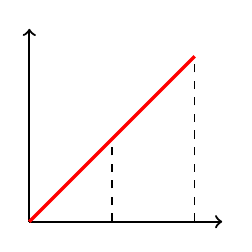
\begin{tikzpicture}[scale=0.7]
\draw[thick,->] (0,0)--(3.5,0);
\draw[thick,->] (0,0)--(0,3.5);
\draw[very thick, red] (0,0)--(3,3);
\draw[dashed] (3,0)--(3,3);
\draw[dashed] (1.5,0)--(1.5,1.5);
\end{tikzpicture}
\end{figure}

Таблица~\ref{tab3} должна иметь номер 3.

\begin{table}[!h]
\caption{Таблица умножения с помощью \texttt{tabularx} (фрагмент)}\label{tab3}
\centering
\begin{tabularx}{\textwidth}{|*{18}{>{\centering\arraybackslash}X|}}\hline
-- & 1 & 2 & 3 & 4 & 5 & 6 & 7 & 8 & 9 & 10 & 11 & 12 & 13 & 14 & 15 & 16 & 17 \\\hline
1  & 1 & 2 & 3 & 4 & 5 & 6 & 7 & 8 & 9 & 10 & 11 & 12 & 13 & 14 & 15 & 16 & 17 \\\hline
2  & 2 & 4 & 6 & 8 & 10 & 12 & 14 & 16 & 18 & 20 & 22 & 24 & 26 & 28 & 30 & 32 & 34 \\\hline
3  & 3 & 6 & 9 & 12 & 15 & 18 & 21 & 24 & 27 & 30 & 33 & 36 & 39 & 42 & 45 & 48 & 51 \\\hline
4  & 4 & 8 & 12 & 16 & 20 & 24 & 28 & 32 & 36 & 40 & 44 & 48 & 52 & 56 & 60 & 64 & 68 \\\hline
\end{tabularx}
\end{table}

\chapterconclusion

В конце каждой главы желательно делать выводы. Вывод по данной главе~--- нумерация работает корректно, ура!


\chapter{Разработка и реализация методов эффективного взаимодействия процессов}

\section{Интерфейс доступа к разрабатываемым методам межпроцессного взаимодествия}

\textbf{TBD: можно взять из бакалаврской ВКР или оставить на нее ссылку.}

Существенная часть межпроцессного взаимодействия - это то, как программист его использует и как сделать это удобным процессом. Интерфейс сокетов в ОС Linux хорошо для этого, так как использует механизм файловых дескрипторов \textbf{TBD: определение или ссылку}, а значит:
\begin{itemize}
\item имеет стандартные примитивы чтения и записи: системные вызовы \textit{read/readv} и \textit{write/writev};
\item позволяет мультиплексировать множество соединений для одновременного отслеживания посредством системных мультиплексоров: \textit{select/poll/epoll}.
\end{itemize}

Удобный и унифицированный интерфейс может объединять под собой совершенно разные методы межпроцессного взаимодействия прозрачным для программиста образом. Программист зачастую не заинтересован в тонкостях передачи данных, ему необходимо реализовывать и совершенствовать пользовательскую логику приложения, однако, поскольку процессы распределенной системы работают вместе над одними задачами, то ему важна и эффективность межпроцессного взаимодействия.

Необходима возможность:
\begin{itemize}
\item предоставлять другим процессам возможность для подключения и подключаться к другим процессам;
\item принимать и передавать данные.
\end{itemize}

Для первого пункта хорошо подходит семейство шаблонов сетевого программирования Acceptor и Connector \cite{schmidt1996acceptor}, которые при необходимости создают экземпляры пользовательских обработчиков соединений, реализующих интерфейс, представленный на Листинге \ref{chapter31:ServiceHandlerInterface}.

\begin{lstlisting}[float=!h,caption={Интерфейс пользовательского обработчика соединений на C++},label={chapter31:ServiceHandlerInterface}]
class ISession
{
public:
	virtual int handle_message(const Message & message) = 0;
	virtual int send(const Message & message) = 0;
	virtual int handle_close() = 0;
};
\end{lstlisting}

%Поскольку существует необходимость полностью оградить программиста от тонкостей работы межпроцессного взаимодействия, чтобы упростить работу пользовательского кода и иметь возможность выбирать наиболее подходящий для данной ситуации метод межпроцессного взаимодействия. выбран событийный асинхронный метод доставки сообщений. Для этого в интерфейсе пользовательского обработчика соединения предусмотрен метод \textit{handle\_message(const Message \&)}. Нижележащая реализация метода межпроцессного взаимодействия вызывает данный метод для соответствующего соединения по факту получения ей очередного сообщения. Для отправки сообщений программисту предлагается использовать примитив \textit{send(const Message \&)}.

\textbf{TBD: кривовато звучит}
Данный интерфейс соответствует асинхронному событийному шаблону проектирования приложений. В этом шаблоне обработчик соединения является пассивной сущностью, в которую события доставляются посредством вызова метода \textit{handle\_message(const Message \&)}. Во-первых, использование этого шаблона позволяет разделить пользовательскую логику и нижележащие методы межпроцессного взаимодействия, работающие по произвольным алгоритмам. Следовательно, это упрощает пользовательскую логику. Во-вторых, позволяет обрабатывать множество соединений числом потоков, не равным количеству этих соединений, так как обработчики соединения нуждаются в потоке для своего выполнения только когда необходимо обработать событие. Для отправки сообщений программисту предлагается использовать примитив \textit{send(const Message \&)}.

Данный интерфейс позволяет скрыть от программиста тонкости работы межпроцессного взаимодействия. Например, отслеживание готовности множества TCP-соединений к передаче или приему данных, состояние соединений. Или то, что взаимодействие происходит через разделяемую память.

\section{Базовый метод межпроцессного взаимодействия на основе TCP}

TCP -- это наиболее широко-используемый и универсальный метод межпроцессного взаимодействия. Протокол гарантирует, что сообщения будут получены в том же количестве и порядке, в котором они были отправлены. Посредством интерфейса сокетов он позволяет взаимодействовать как с локальными, так и с удаленными процессами распределенной системы. Более того, сторонние системы тоже зачастую предоставляют возможность именно подключения по TCP.

Кроме распространенности и удобства для программиста, предоставляют очень важную возможность отслеживания времени жизни соединения. Это важно, так как случае краха процесса операционная система в ходе освобождения системных ресурсов также закроет все TCP-соединения процесса и другие стороны межпроцессного взаимодействия смогут корректно обработать закрытие соединений.

\subsection{Мультиплексирование соединений}

Межпроцессное взаимодействие посредством TCP позволяет использовать системные мультиплексоры событий \textit{select/poll/epoll} для отслеживания событий в множестве TCP-соединений: наличия данных, готовности канала к передаче, закрытия соединения. В системах с большим количеством неактивных соединений лучше всего себя показывает системный мультиплексор \textit{epoll}, при наличии небольшого количества активных соединений большой разницы между ними не наблюдается \cite{MuxComparison}.

Классическим подходом при разработке сетевых приложений является применение шаблона Реактор \cite{schmidt1995reactor, 10.1145/1808954.1808964} для диспетчеризации множества соединений. В настоящей работе используется реализаций шаблона Реактор из библиотеке ACE \cite{ACE}, работающая с системным мультиплексором событий \textit{select}.

Реактор -- это объект, в котором регистрируются обработчики событий и которые Реактор вызывает посредством вызовов их интерфейсных методов. Сокращенный интерфейс обработчика событий из библиотеки ACE приведен в листинге \ref{chapter31:LowLevelServiceHandlerInterface}.
\begin{lstlisting}[float=!h,caption={Интерфейс низкоуровневого обработчика соединений на C++},label={chapter31:LowLevelServiceHandlerInterface}]
class ACE_Event_Handler
{
public:
	virtual int handle_input(ACE_HANDLE fd) = 0;
	virtual int handle_output(ACE_HANDLE fd) = 0;
	virtual int handle_close(ACE_Handle fd, ACE_Reactor_Mask close_mask) = 0;
};
\end{lstlisting}

\textbf{TBD}

\subsection{Обслуживание активных соединений}

\textbf{TBD}

\subsection{Динамическое конфигурирование соединений}
\textbf{TBD: надо написать про стек модулей}


\section{Применение разделяемой памяти для передачи данных}

\textbf{TBD: описать SPSC очередь на буфере постоянного размера}

Однако, недостаточно разместить очередь в разделяемой памяти и отправлять в нее сообщения. Кроме контроля времени жизни соединения, существенный вопрос в данном методе: кто, как и когда будет принимать сообщения. На одном физическом узле может находится множество взаимодействующих процессов с большим количеством соединений между ними. Соответственно, для каждого соединения появляется своя точка синхронизации, в которой процесс-получатель может узнать, что очередь не пуста.

Необходимо разработать метод оповещения процесса-получателя о появлении данных в разделяемой памяти, которые ему необходимо принять и обработать.

\section{Методы оповещения о появлении данных в разделяемой памяти}

\subsection{Наивные алгоритмы в разделяемой памяти}

Процесс-получатель знает о расположении всех очередей в разделяемой памяти, в которые отправляют сообщения все процессы-писатели, с которыми он взаимодействует. Непосредственно само состояние очередей может быть использовано для оповещения процесса-читателя о наличии данных в этих очередях.

\paragraph{Алгоритм №1}

При небольшом количестве соединений (например, $0.25 * N$, где $N$ - количество ядер в процессоре) возможно использование выделенных потоков в процессе-читателе для активного опроса состояния очереди и обработки соответствующего соединения. \textbf{TBD: иллюстрацию?}

\paragraph{Алгоритм №2}

При большем количестве соединений возможно использовать группу выделенных потоков, активно опрашивающих которое количество очередей в разделяемой памяти. Например, 1 поток, постоянно опрашивающий до 10 соединений. \textbf{TBD: иллюстрацию?}

\subsubsection{Применимость, достоинства и недостатки}

Данные алгоритмы активного опроса очередей в разделяемой памяти для обслуживания соединений вполне могут быть использованы в реальных системах. Их можно применить в системах: с большими вычислительными ресурсами, небольшим количеством процессов и очень активных соединений.

В противном случае, активно работающие потоки будут выполнять много бесполезных операций по опросу пустых очередей неактивных соединений. Кроме того, постоянно работающий поток может быть вытеснен с процессора планировщиком операционной системы из-за израсходования отведенного ему кванта процессорного времени.

\subsection{TCP}\label{chapter31:SignalTCP}

Как было сказано выше, TCP используется как базовый метод межпроцессного взаимодействия. Он может быть использован и как метод оповещения о появлении данных в очереди в разделяемой памяти.

\subsubsection{Алгоритм взаимодействия при использовании TCP для оповещения о появлении данных}

\textbf{TBD: нужна иллюстрация взаимодействия и стек модулей}
% Чтобы процесс-получатель о наличии данных в очереди в разделяемой памяти, необходимо:

\begin{enumerate}
\item процессу-получатель ожидает новых данных по всем своим TCP соединениям в состоянии сна в системном мультиплексоре событий;
\item для передачи данных таким методом процессу-отправителю необходимо записать в очередь нужное сообщение и передать на нижележащий модуль сообщение минимального размера в 1 байт с заранее установленным значением (например, ''0``);
\item ядро операционной системы пробуждает процесс-получатель;
\item реактор процесса-получателя демультиплексирует активное TCP соединение, считывает 1 байт полезных данных и отправляет его на следующий слой обработки межпроцессных взаимодействий через ранее описанный стек модулей;
\item модуль, отвечающий за взаимодействие по разделяемой памяти, проверяет, что полученный 1 байт имеет заранее оговоренное значение (''0`` в примере выше) и это служит для него сигналом к проверке состояния очереди в разделяемой памяти для соединения, с которого этот сигнальный байт был получен;
\item процесс-получатель считывает сообщение из очереди и выполняет его обработку.
\end{enumerate}

Таким образом происходит передача данных между процессами в разделяемой памяти с оповещением о появлении данных в разделяемой памяти по TCP.

\subsubsection{Работа с очередью в разделяемой памяти при использовании TCP для оповещения о появлении данных}\label{chapter31:SharedMemoryOptimization}

\textbf{TBD: module stack, handshake}
\textbf{TBD: нужна иллюстрация взаимодействия или какой- нибудь псевдокод}

\subsubsection{Достоинства и недостатки}

Предложенный метод обладает следующими \textbf{достоинствами}:
\begin{itemize}
\item позволяет эффективно поддерживать множество соединений с использованием системных мультиплексоров событий (\textit{select/poll/epoll});
\item позволяет процессу-получателю блокировать свое выполнение до появления оповещения;
\item благодаря использованию эвристики из раздела \ref{chapter31:SharedMemoryOptimization} временная задержка на передачу данных может быть снижена, если к концу обработки очередного сообщения в очередь уже будет записано новое сообщение;
\item метод межпроцессного взаимодействия по TCP не требует доработки и может быть использован как есть.
\end{itemize}

\textbf{Недостаток} у такого подхода только один: временная задержка на отправку и получение оповещения. Основные отличия от метода, использующего только TCP, в том, как передается само сообщения. Но кроме использования среды для передачи самих данных выполняется рад системных вызовов для оповещения процесса-читателя, каждый из которых может вносить существенную временную задержку:
\begin{itemize}
\item \textit{write} -- для записи 1 байта в TCP-сокет процессом-писателем;
\item \textit{select/poll/epoll} -- для демультиплексирования нужного события среди множества источников процессом-читателем.
\item \textit{read} -- для чтения 1 байта из TCP-сокета процессом-читателем.
\end{itemize}

В случае, когда процесс-получатель находится в состоянии сна на системном мультиплексоре событий, процесс-отправитель в ходе системного вызова \textit{write} должен также изменить состояние процесса-получателя на ''Готов к выполнению`` или ''Выполняется``. После этого в течение некоторого промежутка времени процесс-получатель будет готовиться к выполнению. Все это может влиять на временную задержку на передачу данных.

Следовательно, необходимо разработать новый метод мультиплексирования соединений, использующих разделяемую память, имеющий меньшие накладные расходы на использование и обладающий, как минимум, теми же достоинствами, что и описанный в данном разделе. 

\subsection{Мультиплексор событий в разделяемой памяти}\label{chapter31:Mux}

С целью избежать излишних накладных расходов и использовать системные ресурсы наилучшим образом в настоящей работе предлагается метод мультиплексирования событий от множества соединений, использующих разделяемую память для передачи данных.

Мультиплексор событий в разделяемой памяти -- это структура данных, используемая множеством процессов-отправителей для оповещения процесса-получателя о появлении данных в очереди в разделяемой памяти. Каждый процесс, участвующий в межпроцессном взаимодействии, должен иметь свой мультиплексор событий.

Время жизни мультиплексора событий определяется процессом-читателем. При необходимости процесс-читатель создает файл определенного размера в ФС и отображает его в свою память. Во время установления соединения процесс-читатель ассоциирует соединение с номером от 0 до 2047 и отправляет его вместе с путем до файла другой стороне. Эти данные используются противоположной стороной для отправки оповещений.

\textbf{TBD: нарисовать схему с двумя процессами и файлом, отображенным в их памяти}

\subsubsection{Структура и алгоритм работы мультиплексора событий в разделяемой памяти}\label{chapter31:MuxStructure}

Структура мультиплексора событий представлена на Рисунке \ref{chapter31:MuxZeroState}. Он состоит из 4-байтного целого числа futex, используемого для синхронизации взаимодействующих процессов, и массив из 32 8-байтных сигнальных чисел, по одному на каждый бит futex. Эти 32 8-байтных числа содержат 2048 бит, что позволяет различать 2048 различных соединений. Описание на языке C++ представлено на Листинге \ref{chapter31:MultiplexerStruct}.


\begin{figure}[!h]
\caption{Структура мультиплексора событий в разделяемой памяти}
\label{chapter31:MuxZeroState}
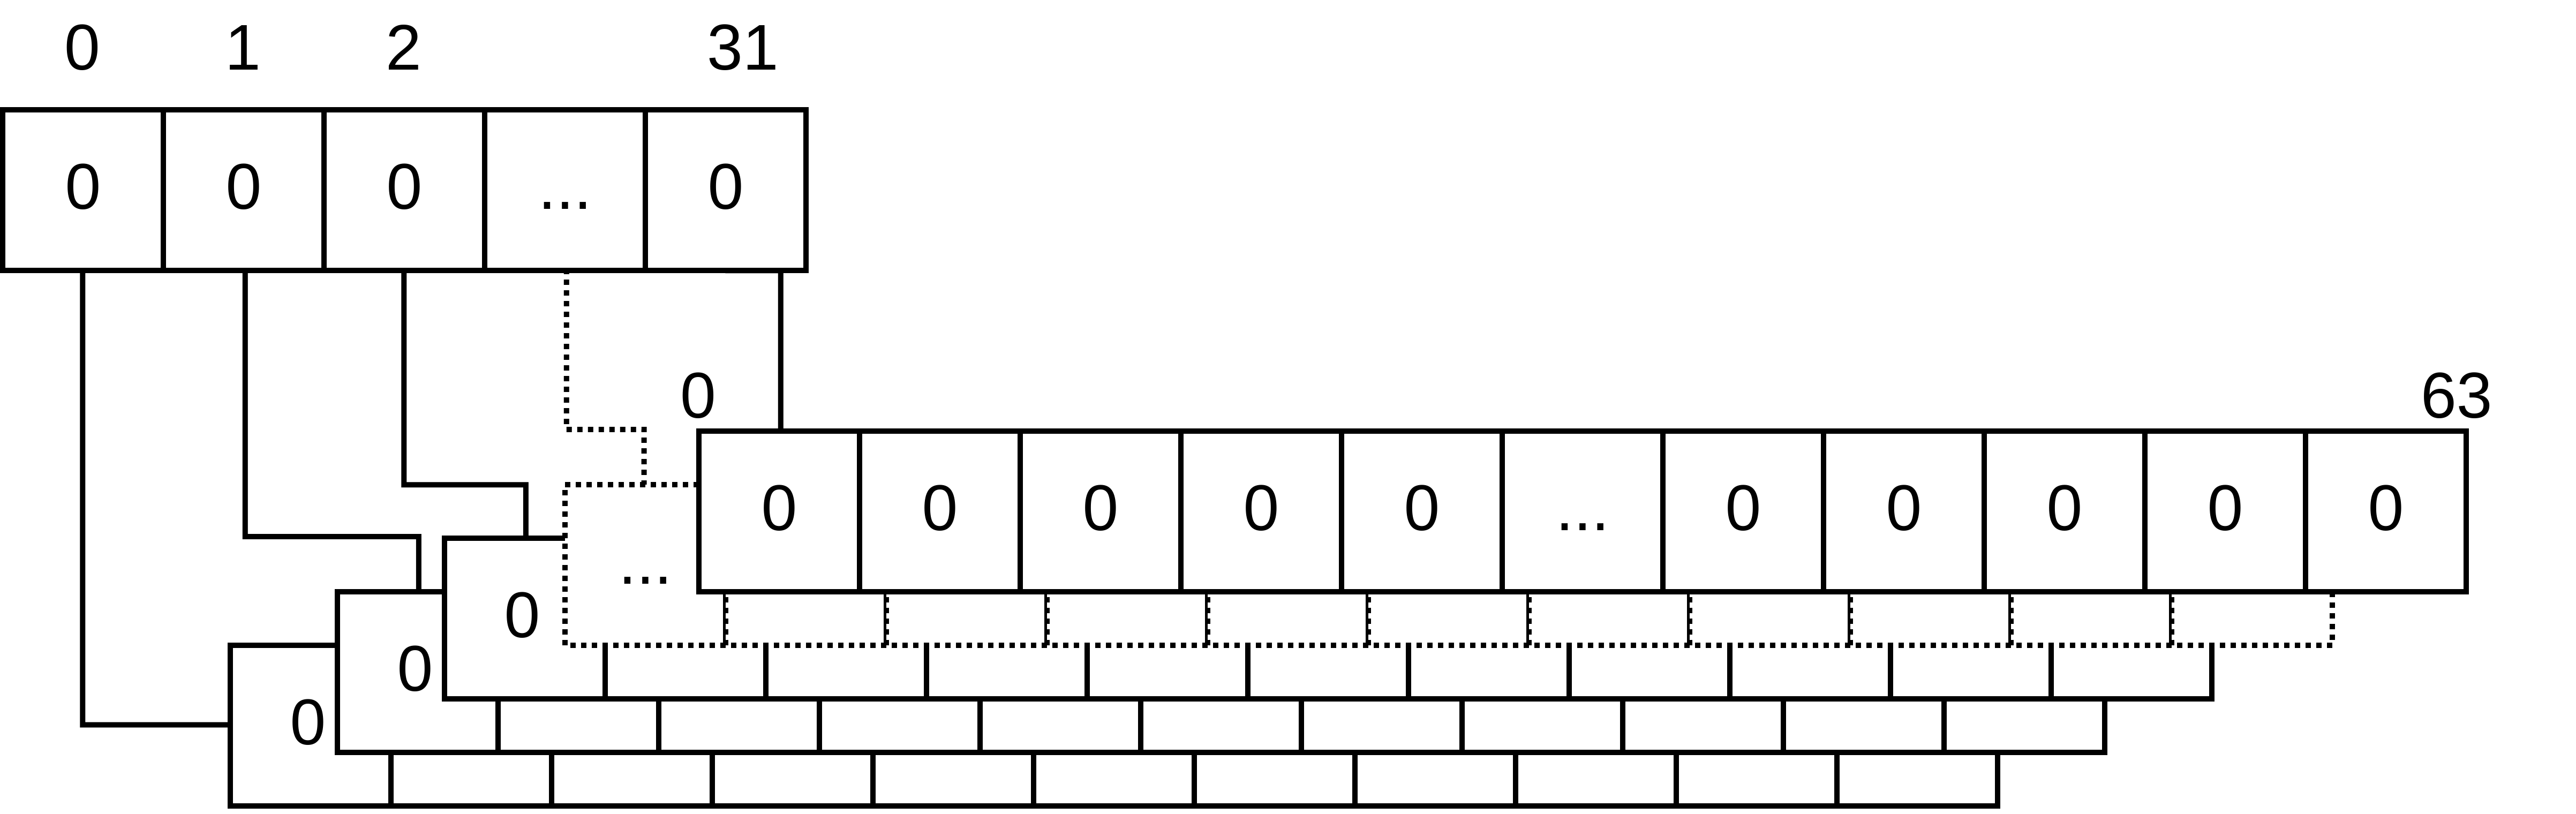
\includegraphics[width=\textwidth]{../../graphics/schemes/futex}
\end{figure}

\begin{lstlisting}[float=!h,caption={Структура мультиплексора в памяти},label={chapter31:MultiplexerStruct},frame=tlrb]
struct Multiplexer
{
    using Futex = std::atomic<int32_t>;
    using Signal = uint64_t;

    static constexpr std::size_t c_num_chunks = sizeof(Futex) * CHAR_BIT;
    static constexpr std::size_t c_signals_per_chunk = sizeof(std::atomic<Signal>) * CHAR_BIT;
	
	// Процедура ожидания на futex
    void wait() {
    	if (!m_futex) {
   			futex_wait(&m_futex, 0);
   		}
    }
	
	// Процедура оповещения процесса-читателя. Выставляет соответствующие биты мультиплексора для сигнала за номером signal и при необходимости пробуждает поток мультиплексора процесса-читателя.
    void notify(Multiplexer::Signal id);
    
    // Процедура для пробуждения потока, спящего на futex.
    void wakeup();

protected:
	// 4-байтное число futex, на котором происходит синхронизация сна/пробуждения потока мультиплексора.
    Futex m_futex;
	
	// Для избежания лишней состязательности между атомарными операциями над массивом сигнальных чисел и над futex, массив выровнен на размер кэш-линии процессора -- 64 байта.
    alignas(64) std::array<std::atomic<Signal>, c_num_chunks> m_signals;
};
\end{lstlisting}

Когда процесс-отправитель хочет оповестить процесс-читатель о наличии данных в очереди в разделяемой памяти, ему необходимо:
\begin{enumerate}
\item атомарно выставить бит в сигнальном числе, соответствующий этому соединению;
\item атомарно выставить соответствующий бит futex и получить его предыдущее значение;
\item Если предыдущее значение равно нулю, значит, разбудить процесс-читатель, чтобы он мог обработать оповещение.
\item Если оно не равно нулю, это значит, что кто-то уже либо разбудил процесс-читатель, либо в скором времени сделает это.
\end{enumerate}

После завершения первых двух этапов мультиплексор для соединения под номером \#1987 будет находиться в состоянии, представленном на рисунке \ref{chapter31:Mux1987State}. Чтобы проставить нужные биты для данного, процесс-отправитель делит номер его соединения на 64 и получает индекс бита в futex -- 31, и, соответственно, индекс сигнального числа. Далее он вычисляет остаток от деления номера сигнала на 64 и получает индекс бита в сигнальном числе. После чего атомарной операцией ''ИЛИ`` выставляется сначала нужный бит в сигнальном числе, а потом нужный бит в futex. Псевдокод алгоритмов процесса-отправителя и получателя приведены на Листингах \ref{appendix91:SignalCode} и \ref{appendix91:ReceiverCode}.

\begin{figure}[!h]
\caption{Состояние мультиплексора событий в разделяемой памяти с активным сигналом \#1987}
\label{chapter31:Mux1987State}
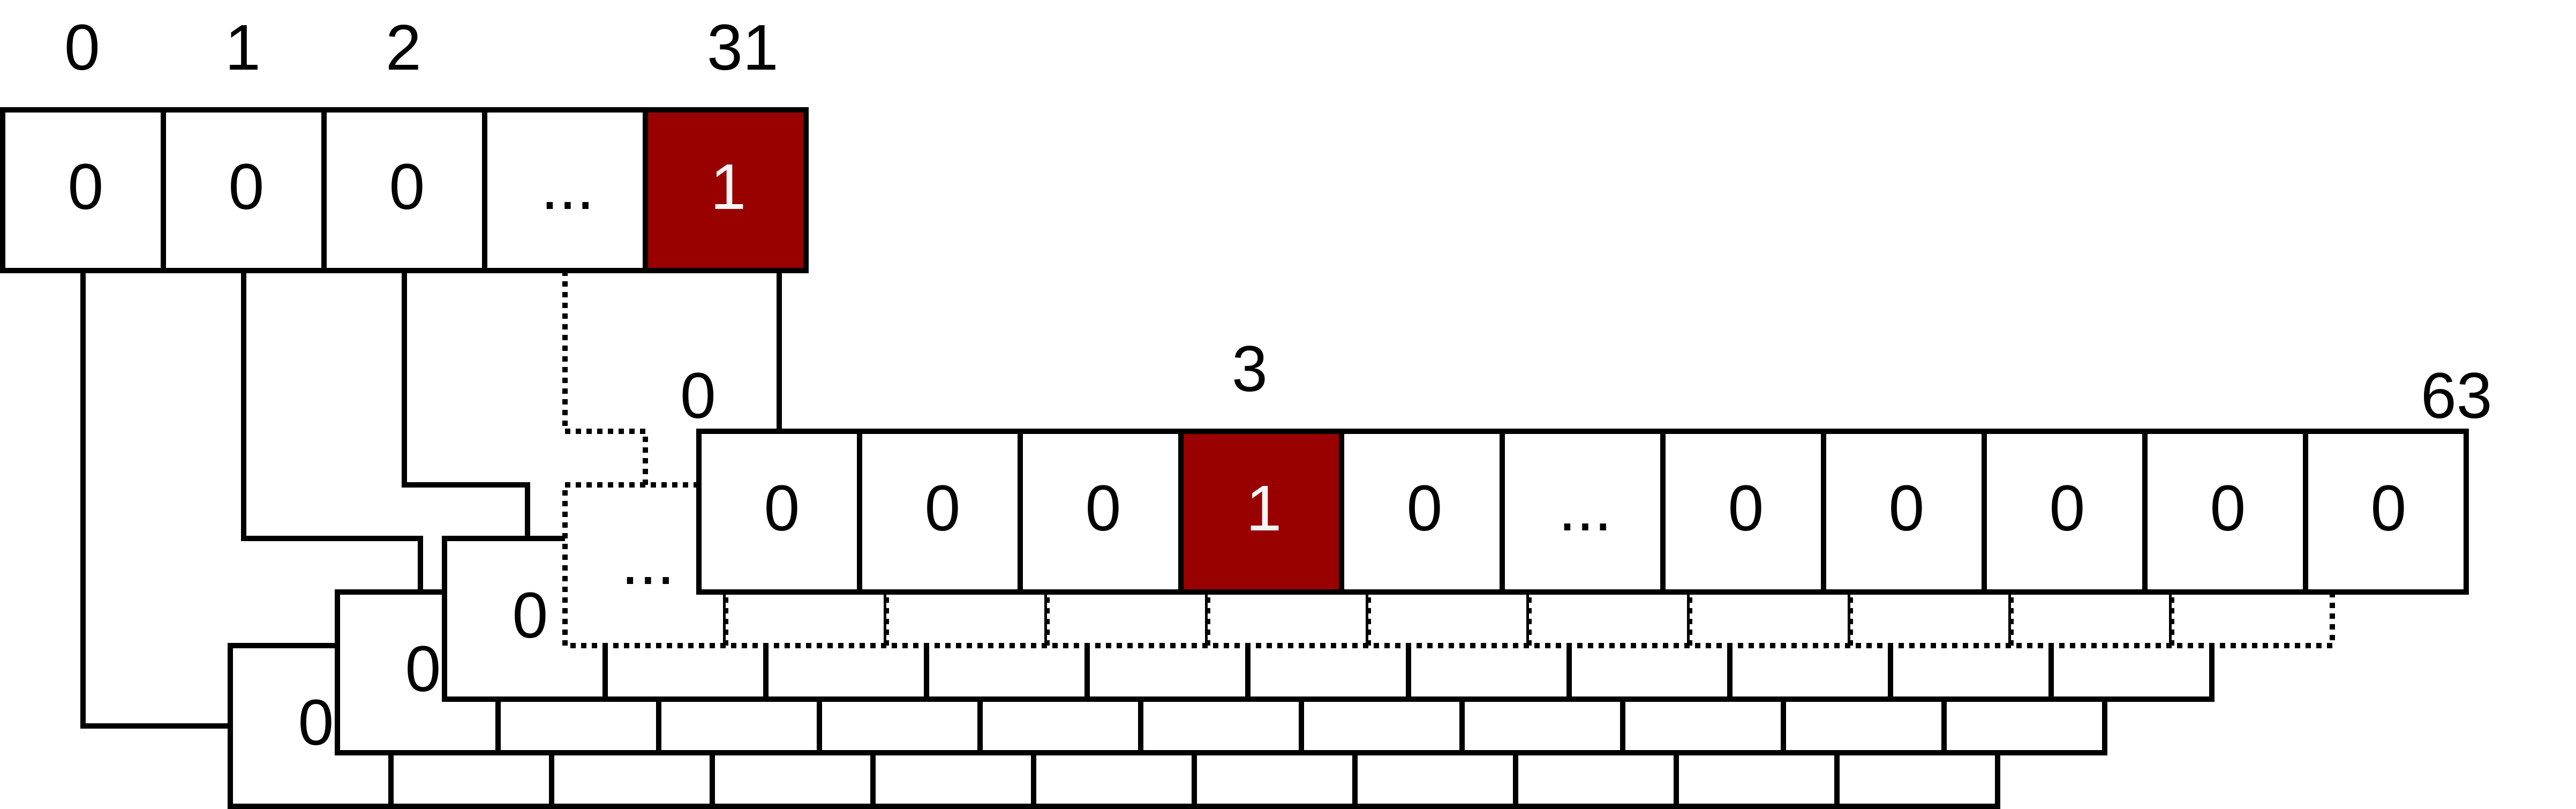
\includegraphics[width=\textwidth]{../../graphics/schemes/futexready}
\end{figure}

\subsubsection{Достоинства и недостатки}

По сравнению с вышеописанным методом, использующим TCP, данное решение обладает следующими \textbf{достоинствами}:
\begin{enumerate}
\item Подавляющая часть работы происходит в пользовательском пространстве. В лучшем сценарии отправка и получение оповещения не задействуют системные вызовы. Оповещение происходит посредством двух атомарных операций.
\item Ядро ОС используется только пробуждения и засыпания процессов.
\end{enumerate}

Таким образом, в худшем случае совершается один системный вызов для засыпания процесса в ожидании оповещений и один для пробуждения процесса. Пробуждение потока влечет временные затраты как со стороны процесса-отправителя -- на пробуждение потока, так и со стороны процесса-получателя -- на уход в состояние сна и временную задержку на постановку потока мультиплексора на выполнение. В то же время, ожидание оповещений в состоянии сна позволяет экономить ресурс процессора.

\textbf{Недостатком} данного метода является механизм управление файлом мультиплексора событий в файловой системе. Поскольку файлом управляет процесс, то в случае его некорректного завершения файл не будет удален и останется на всегда. Некорректное завершение может произойти по следующим причинам: крах процесса вследствие программного дефекта, при отправке сигнала \textit{SIGKILL} процессу, который в большинстве случаев приводит к немедленному завершению процесса.

Данный недостаток можно решить, используя более продвинутый механизм создания файлов в ФС. Например, делегировать эту работу отдельному процессу или группе процессов. В таком случае такой процесс может отслеживать состояние своих клиентских процессов и при прекращении их работы выполнять подчистку ресурсов.

\subsection{Методы обработки оповещений в мультиплексоре событий}

Имея более совершенный механизм оповещения процессов о появлении данных в разделяемой памяти необходимо разработать также и метод обработки получаемых оповещений. В данном подразделе предложены четыре метода:
\begin{enumerate}
\item Синхронный -- существует единственный выделенный поток мультиплексора. Он занимается непосредственно обслуживанием соединений.
\item ''Полусинхронный/Полуреактивный`` -- существует единственный выделенный поток мультиплексора (полуреактивная часть). Он диспетчеризует синхронную обработку оповещений в пул потоков (полусинхронная часть) \cite{schmidt1995half}.
\item ''Лидер/Последователи`` -- в один момент времени только один поток-лидер отслеживает состояние мультиплексора в блокирующем режиме. То есть, при отсутствии оповещений процесс-лидер находится в состоянии сна. При обнаружении оповещений он передает лидерство произвольному потоку из пула и переходит к обработке оповещений \cite{schmidt1998leader}.
\item ''Лидер/Последователи`` -- в один момент времени только один поток-лидер активно отслеживает состояние мультиплексора. То есть, постоянно опрашивает мультиплексор. При обнаружении оповещений он передает лидерство произвольному потоку из пула и переходит к обработке оповещений \cite{schmidt1998leader}.
\end{enumerate}

\subsubsection{Синхронный метод обработки соединений}

\subsubsection{Метод обработки соединений ''Полусинхронный/Полуреактивный``}\label{chapter31:BlockingHSHA}
Описан в ранней работе \cite{GubarevFutex} автора.

\subsubsection{Метод обработки соединений ''Лидер/Последователи``}\label{chapter31:BlockingLF}

\subsubsection{Метод обработки соединений ''Лидер/Последователи`` с активным ожиданием оповещений}\label{chapter31:NonBlockingLF}

\chapterconclusion

\textbf{TBD: Вывод по очередной главе}


\chapter{Экспериментальное исследование и обработка результатов}\label{chapter41}

\section{Постановка эксперимента}

\subsection{Конфигурация экспериментального стенда}

\subsubsection{Аппаратное обеспечение}

Процессоры 2 x Intel Xeon Platinum 8168 CPU @ 2.7 GHz.
Технология Hyper-Threading отключена для уменьшения нежелательного влияния на время обслуживания заявок в системе \cite{LowLatencyHT}.

Оперативная память: DDR4-2666 128 GiB.

\subsubsection{Программное обеспечение}

Операционная система Red Hat Enterprise Linux Server release 7.8 (Maipo).
Ядро Linux 3.10.0-1127.el7.x86\_64

Компилятор C++ Clang 6.0.1.

Стандартная библиотека C++: libstdc++ 8.1.0.

Библиотека Boost.Interprocess 1.68.0.

\subsection{Конфигурация экспериментальной системы}

Система для проведения эксперимента состоит из двух процессов:
\begin{itemize}
\item Процесс-шлюз отвечает за преобразование заявок из формата внешнего мира во внутренний формат системы и обратно. 
\item Процесс-обработчик совершает некоторые преобразования над заявкой и отправляет результат за пределы системы через процесс-шлюз.
\end{itemize}

Процессы выполняются на двух процессорах, расположенных в разных разъемах на материнской плате физического узла.

Снаружи системы находится симулятор внешнего мира. Он генерирует поток заявок в систему и получает результат обработки заявки в системе. Схема взаимодействия процессов в эксперименте представлена на рисунке \ref{chapter41:SystemSchema}.

\begin{figure}[!h]
\caption{Схема взаимодействия процессов в эксперименте}
\label{chapter41:SystemSchema}
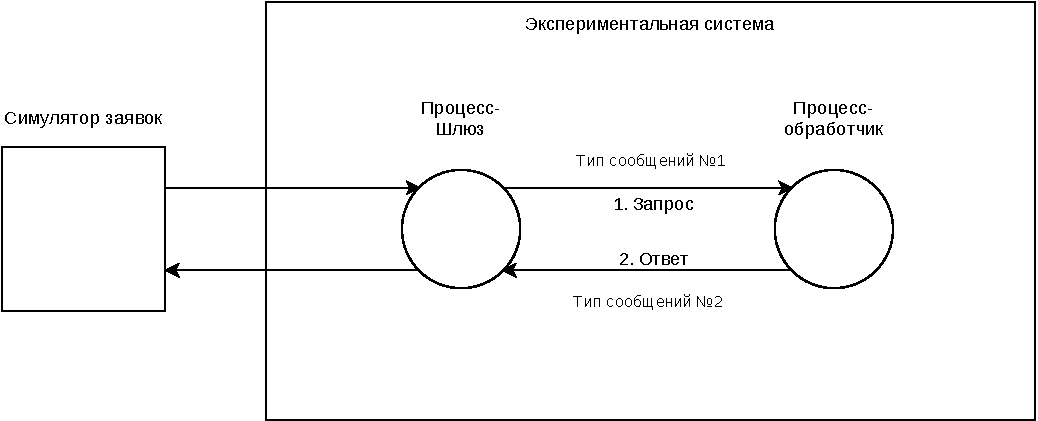
\includegraphics[width=\textwidth]{../../graphics/schemes/SystemSchema}
\end{figure}

В настоящей работе замеряется временная задержка на передачу данных между процессами внутри системы, а именно из процесса-шлюза в процесс-обработчик и обратно (сообщения типа №1 и №2 в запросе и ответе между процессом-шлюзом и процессом обработчиком на рисунке \ref{chapter41:SystemSchema}).

Процессы системы взаимодействуют используют одно соединение, в рамках которого заявки обрабатываются строго последовательно.
Обслуживание включает в себя: прием заявки, выполнение пользовательской логики над заявкой и, если необходимо, отправка ответа.
Временной задержкой на передачу данных в настоящей работе принимается временной промежуток от начала отправки заявки до \textbf{начала обработки заявки}. Таким образом, возможен случай, когда во время обработки очередной заявки процессом в очереди уже находится следующая заявка, временная задержка на передачу которой, таким образом, увеличится на время обработки текущей заявки.

Данный сценарий актуален для процесса-обработчика, в котором обслуживание заявки осуществляется непосредственно в транспортном потоке
В случае с процессом-шлюзом транспортный поток только читает и диспетчеризует асинхронную обработку заявки, т.е. не выполняет обработку самой заявки.

\textbf{TBD: надо как- то адекватно это описать}
Пользовательская логика процесс-обработчика в среднем отклоняет 25\% заявок, в то время как 75\% заявок отправляются в процесс-шлюз.

\subsection{Используемые обозначения}

\begin{itemize}
\item $\Delta$ -- временная задержка между сериями заявок;
\item $\delta$ -- временная задержка между заявками в серии;
\item $\tau$ -- временная задержка на передачу данных;
\item $T$ -- время обслуживания заявки.
\item транспортный поток -- поток из пула транспортных потоков, непосредственно обслуживающий получаемые заявки.
\end{itemize}

Из-за сложного характера распределений для представления полученных данных используются гистограммы выборок и 50, 80, 90, 95 и 99 процентили.

\subsection{Характер экспериментальной нагрузки}

Характеристики потока заявок, создаваемого симулятором, приведены в таблице \ref{chapter41:TableSimulator}.
\begin{table}[!h]
\caption{Процентили интервалов между сериями заявок и заявками, создаваемыми симулятором}\label{chapter41:TableSimulator}
\centering
\begin{tabular}{|l|l|l|l|l|l|l|l|}
\hline
Процентиль & 0\% & 50\% & 80\% & 90\% & 95\% & 99\% & 100\% \\ \hline
$\Delta$, мс & 5 & 9 & 11 & 12.5 & 13 & 15 & 109 \\ \hline
$\delta$, мкс & 52 & 62 & 82 & 110 & 115 & 128 & 4819 \\ \hline
\end{tabular}
\end{table}

\subsection{Время обслуживания заявок в процессах}

На рисунке \ref{chapter41:EngineLatency} представлена гистограмма времени обслуживания заявок в процессе-обработчике. В таблице \ref{chapter41:TableEngine} представлены процентили времени обслуживания заявок в процессе-обработчике.
\begin{figure}[!h]
\caption{Гистограмма времени обслуживания заявки в процессе-обработчике}
\label{chapter41:EngineLatency}
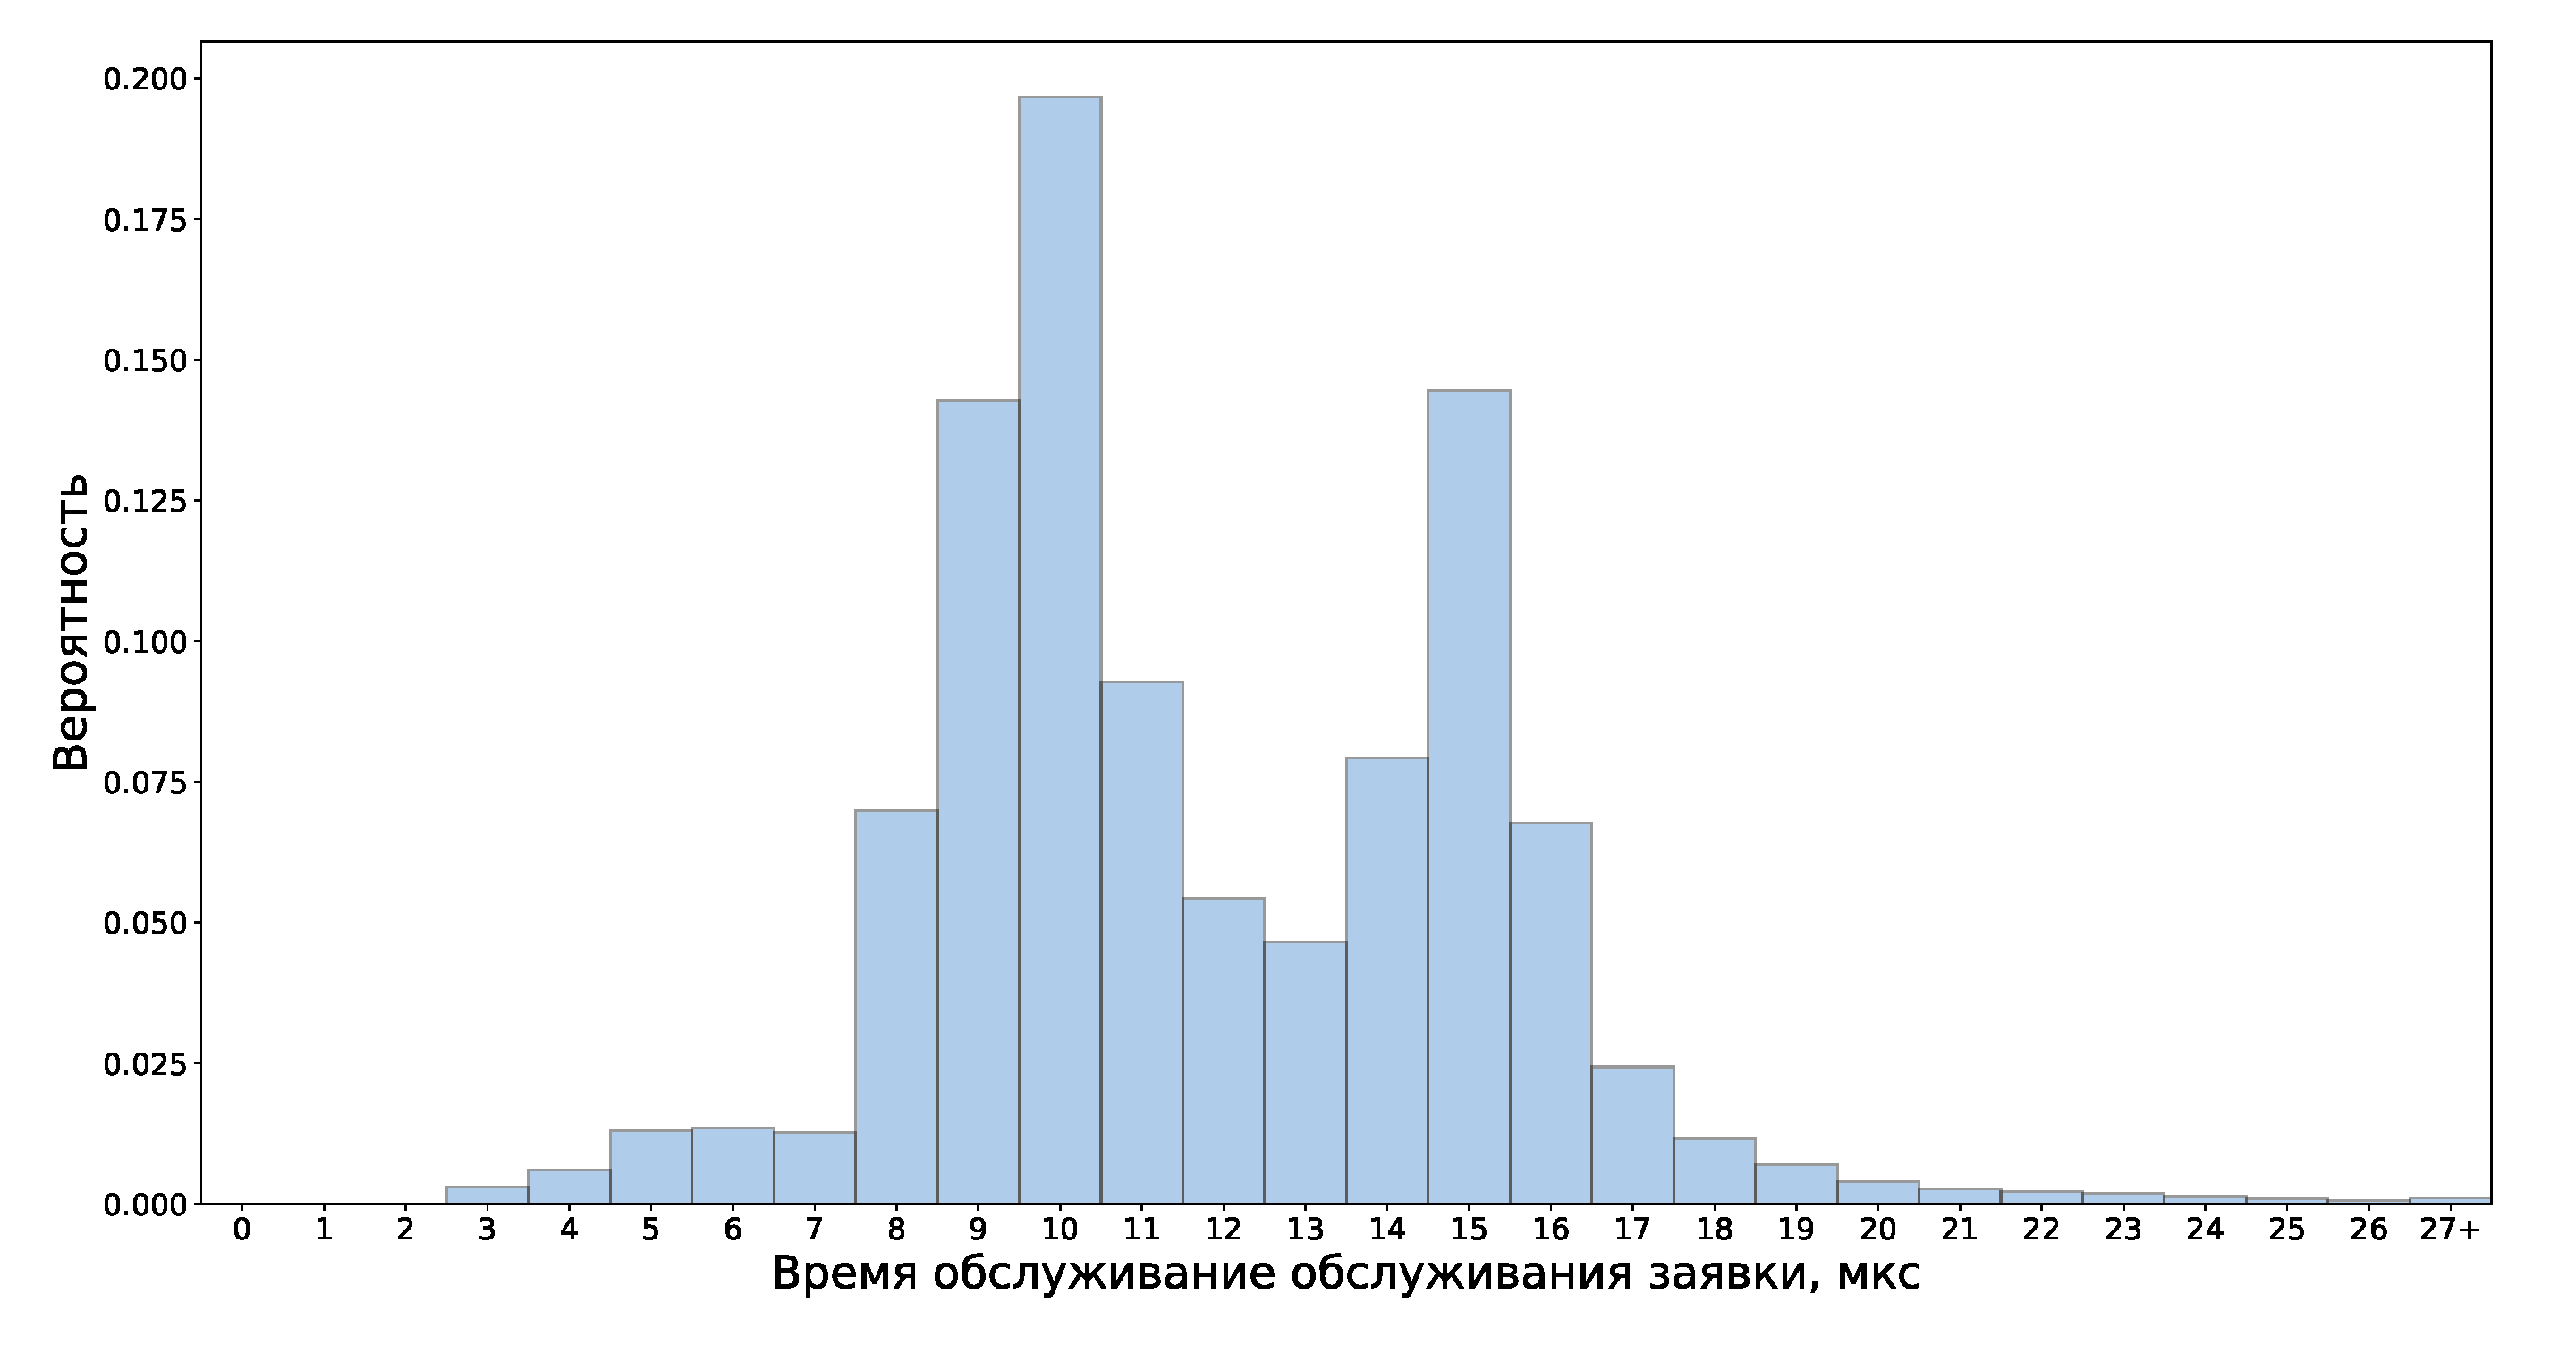
\includegraphics[width=\textwidth]{../../graphics/hist/Engine}
\end{figure}

\begin{table}[!h]
\caption{Процентили времени обслуживания заявок в процессе-обработчике}\label{chapter41:TableEngine}
\centering
\begin{tabular}{|l|l|l|l|l|l|l|l|}
\hline
Процентиль & 0\% & 50\% & 80\% & 90\% & 95\% & 99\% & 100\% \\ \hline
$T$, мкс & 2 & 11 & 15 & 16 & 17 & 21 & 285 \\ \hline
\end{tabular}
\end{table}

На рисунке \ref{chapter41:TRLatency} представлена гистограмма времени обслуживания заявок в процессе-шлюзе. В таблице \ref{chapter41:TableTR} представлены процентили времени обслуживания заявок в процессе-обработчике.
\begin{figure}[!h]
\caption{Гистограмма времени обслуживания заявки в процессе-шлюзе}
\label{chapter41:TRLatency}
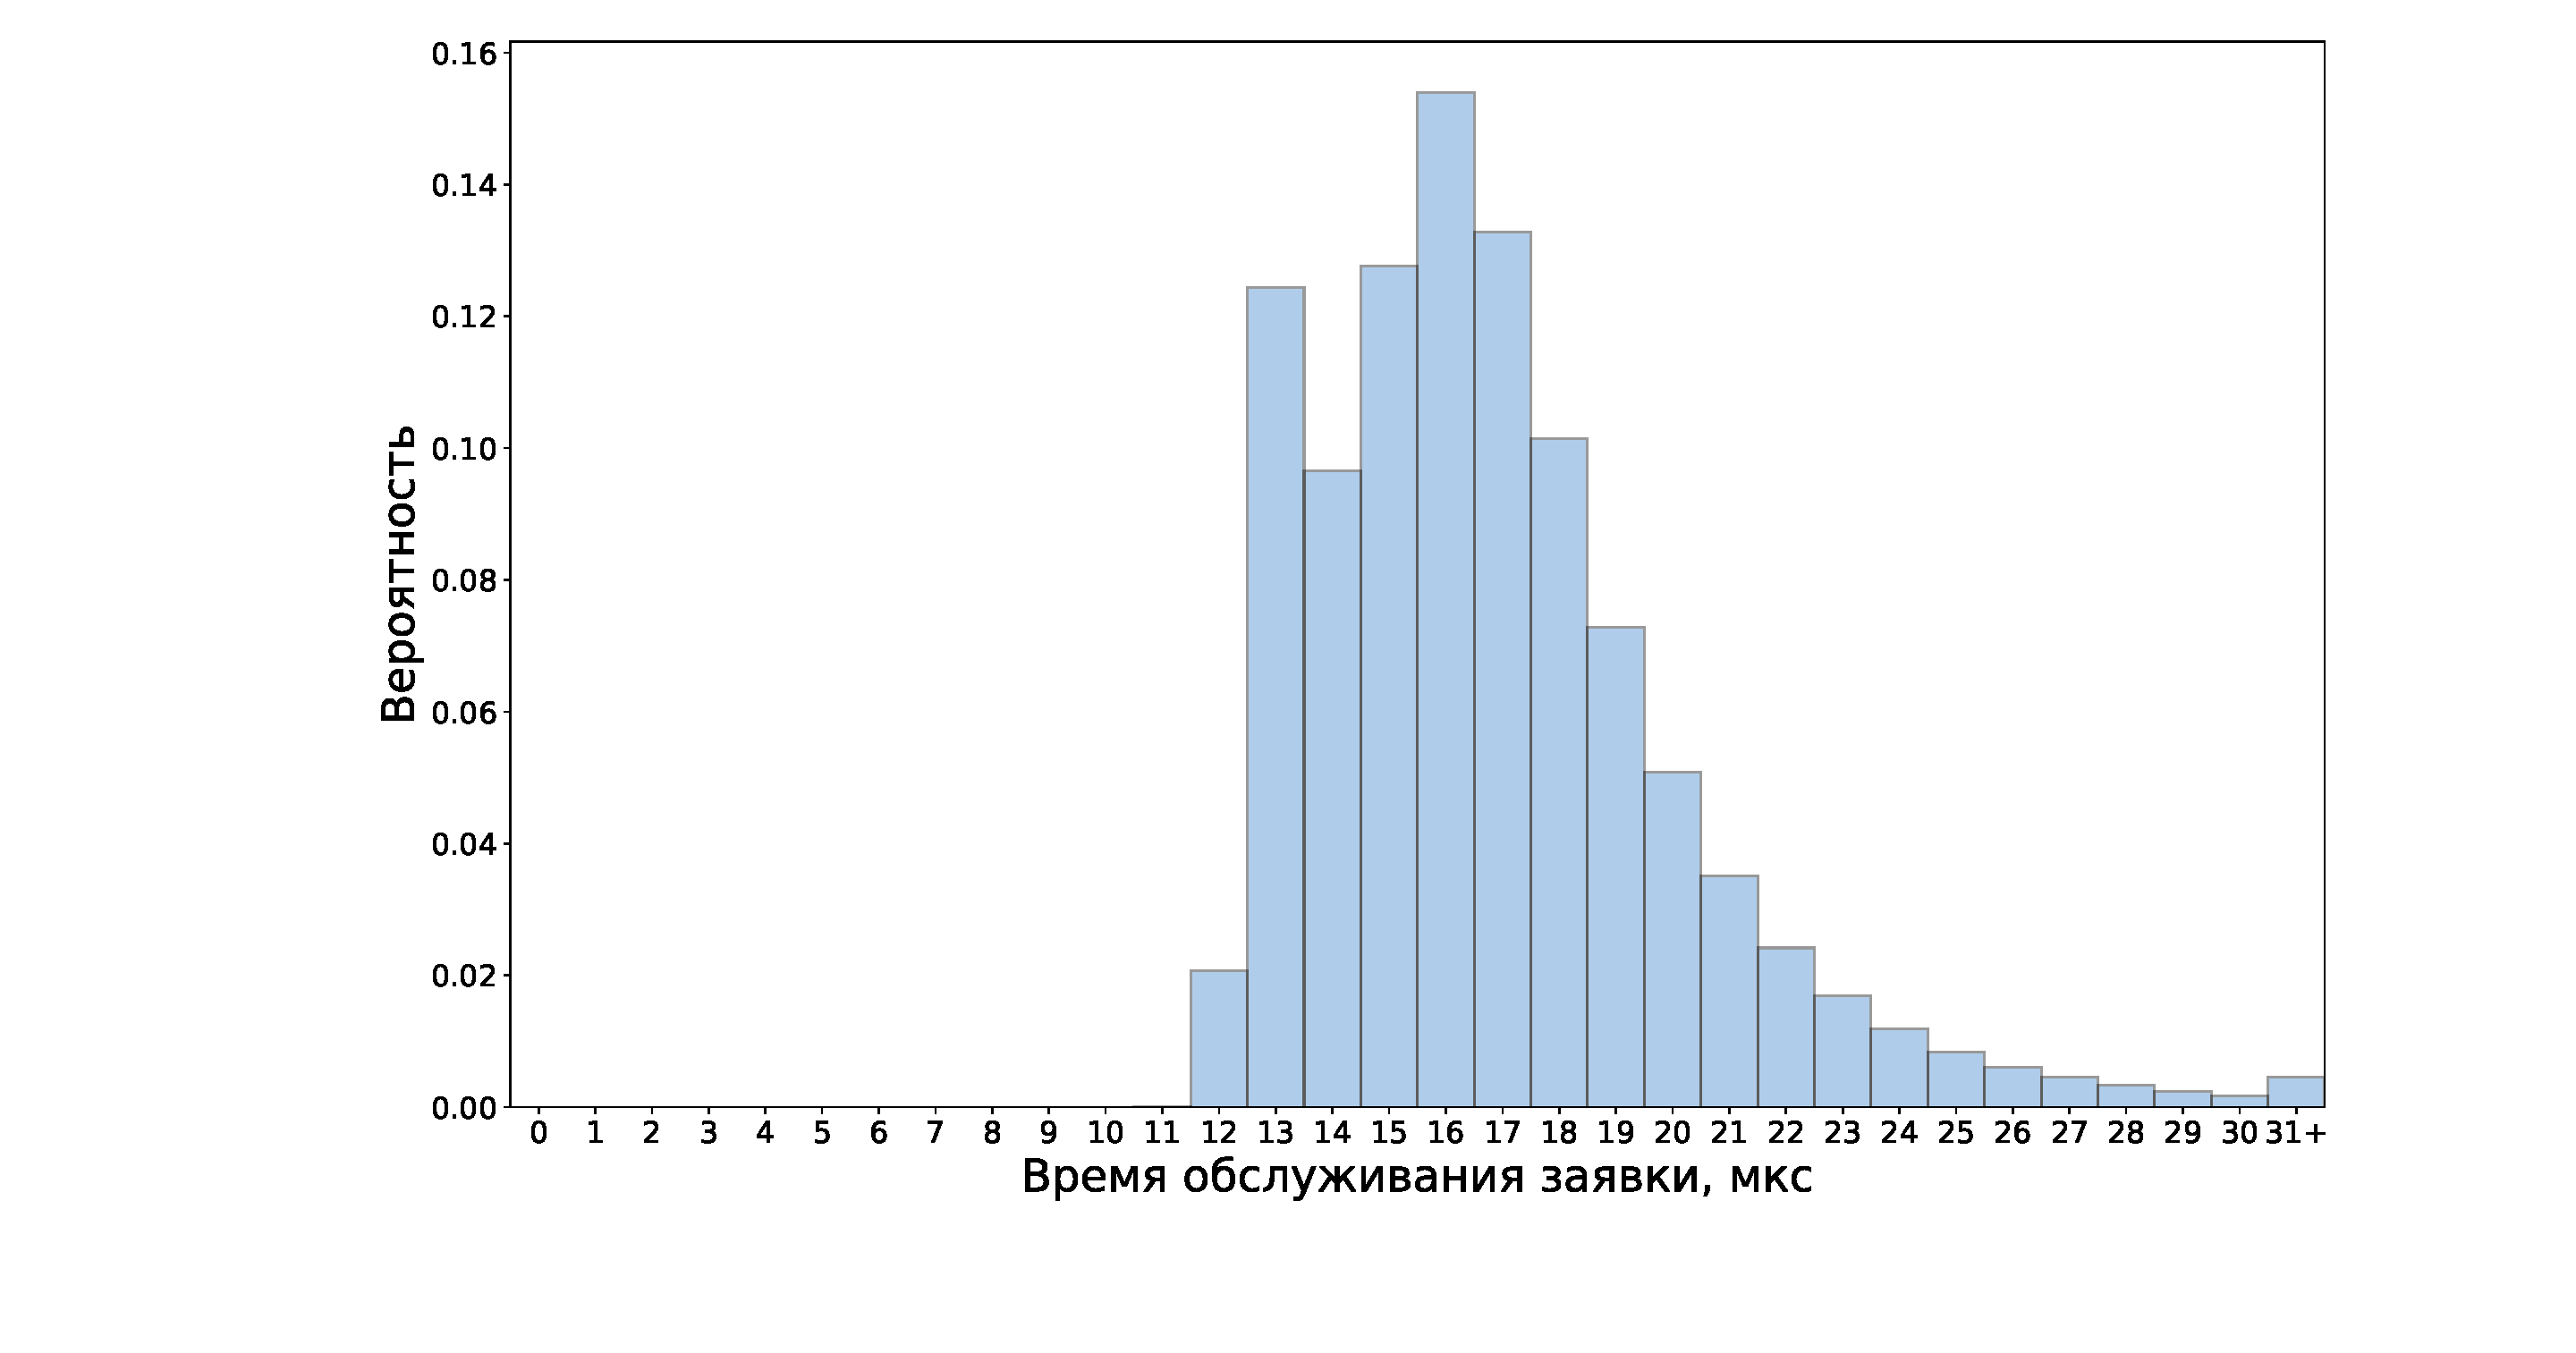
\includegraphics[width=\textwidth]{../../graphics/hist/TR}
\end{figure}

\begin{table}[!h]
\caption{Процентили времени обслуживания заявок в процессе-шлюзе}\label{chapter41:TableTR}
\centering
\begin{tabular}{|l|l|l|l|l|l|l|l|}
\hline
Процентиль & 0\% & 50\% & 80\% & 90\% & 95\% & 99\% & 100\% \\ \hline
$T$, мкс & 11 & 16 & 19 & 21 & 23 & 27 & 5678 \\ \hline
\end{tabular}
\end{table}

\textbf{TBD: а надо ли мне вообще говорить тогда про время обслуживания заявок в процессе-шлюзе? Может, убрать совсем?}
Как было сказано выше, в процессе-шлюзе заявки обслуживания вне транспортного потока, поэтому время обслуживания заявок в процессе-шлюзе не влияет на временную задержку на передачу данных. В случае с процессом-обработчиком значительная часть обслуживания заявки выполняется именно в транспортном потоке, что влияет на временную задержку на передачу данных, т.к. нахождение в очереди на обслуживание влияет на данный показатель.


\section{Использование TCP для передачи данных}


В качестве точки отсчета в настоящей работе выступает метод межпроцессного взаимодействия на основе TCP, используемый посредством сокетов \textbf{TBD: ссылка на определение и на раздел диссертации} \ref{chapter31:PureTCP}.

Показатели потока исходящих заявок из симулятора в данном эксперименте: $\Delta \in$ \textit{10 $\pm$ 4 мс}, $\delta \in$ \textit{50 $\pm$ 26 мкс}.

\begin{figure}[!h]
\caption{Гистограмма временной задержки на передачу данных между процессами при использовании TCP}
\label{chapter41:FigPureTCP}
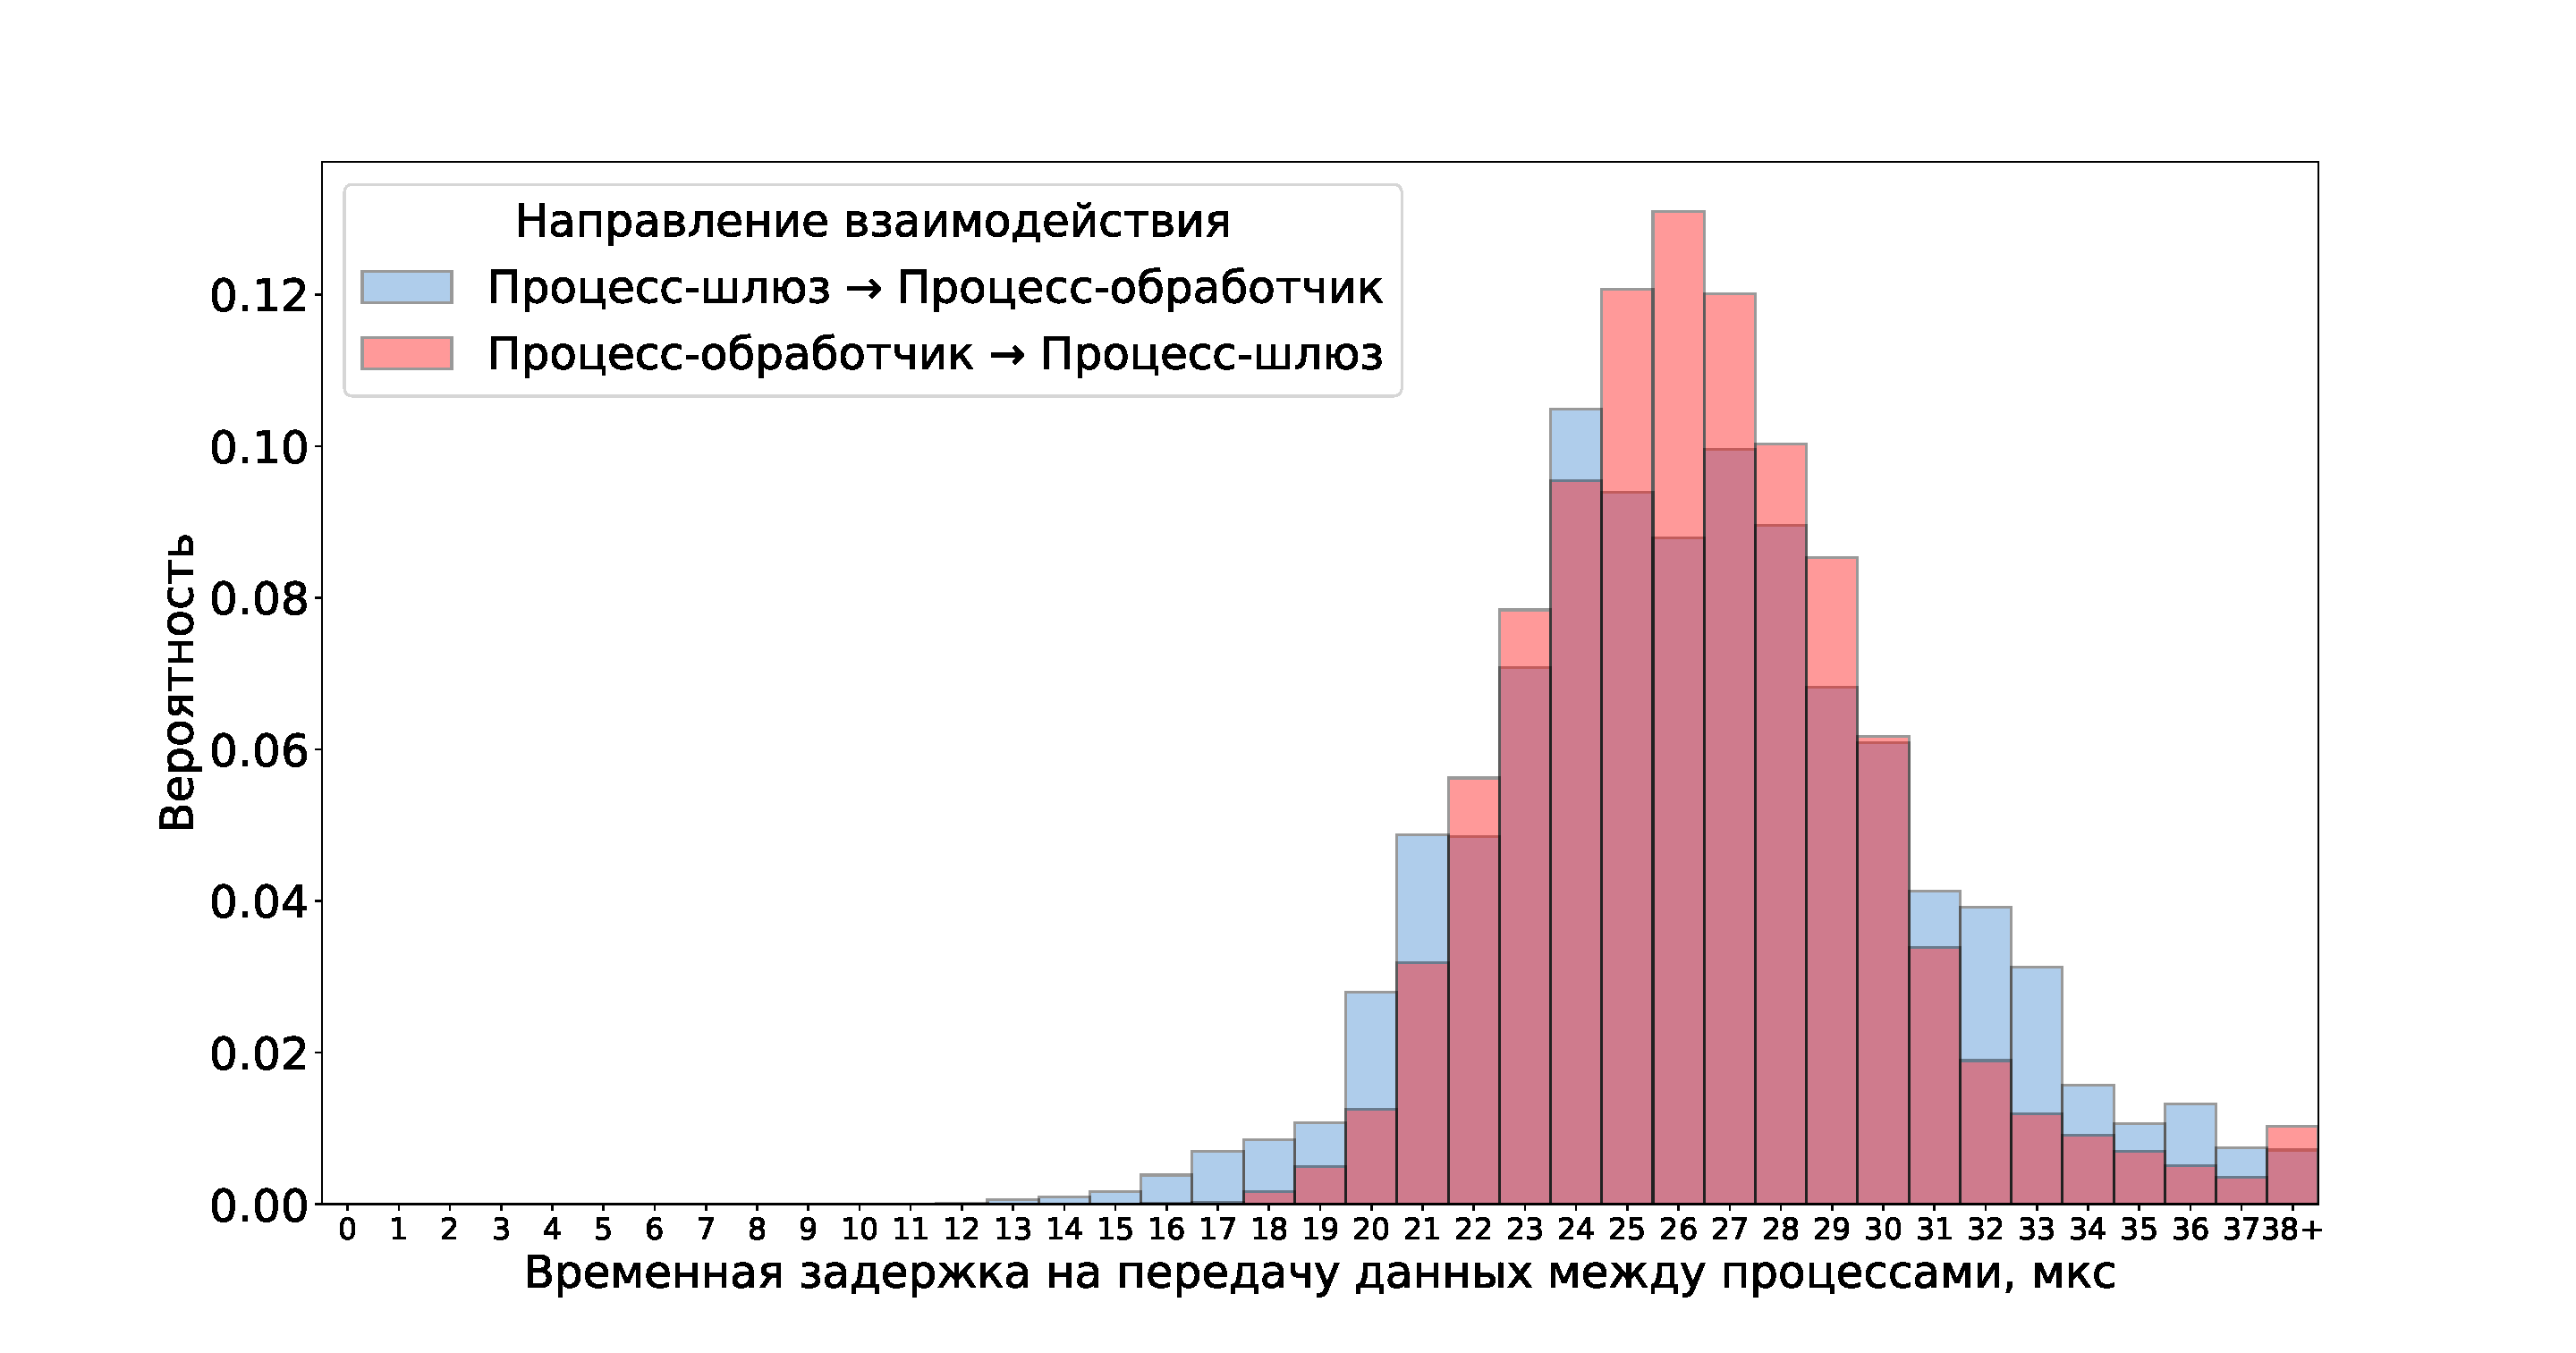
\includegraphics[width=\textwidth]{../../graphics/hist/PureTCP}
\end{figure}

Гистограмма временной задержки на передачу данных для данного метода приведена на Рисунке \ref{chapter41:FigPureTCP}. В Таблице \ref{chapter41:TablePureTCP} приведены основные временные характеристики данного метода.

\begin{table}[!h]
\caption{Основные показатели временной задержки на передачу данных для метода на основе TCP}\label{chapter41:TablePureTCP}
\centering
\begin{tabular}{|l|c|c|}
\hline
\begin{tabular}[c]{@{}l@{}}Направление\\ взаимодействия/\\ Показатель\end{tabular} & \multicolumn{1}{l|}{\begin{tabular}[c]{@{}l@{}}Процесс-шлюз $\rightarrow$\\ Процесс-обработчик\end{tabular}} & \multicolumn{1}{l|}{\begin{tabular}[c]{@{}l@{}}Процесс-обработчик $\rightarrow$\\ Процесс-шлюз\end{tabular}} \\ \hline
min(t), мкс & 9 & 13 \\ \hline
M(t), мкс & 27.5 $\pm$ 8.5 & 28 $\pm$ 7 \\ \hline
max(t), мс & 2.1 & 9.2 \\ \hline
\begin{tabular}[c]{@{}l@{}}$\Delta$, мс\end{tabular} & 10 $\pm$ 4 & 10 $\pm$ 4 \\ \hline
\begin{tabular}[c]{@{}l@{}}$\delta$, мкс\end{tabular} & 50 $\pm$ 26 & 87 $\pm$ 32 \\ \hline
\end{tabular}
\end{table}

Временная задержка на передачу данных в обоих направлениях имеет схожие значения. Это объясняется тем, что накладные расходы на использование TCP через механизм сокетов имеют подавляющее значение над прочими факторами, влияющими на межпроцессное взаимодействие.

\section{Использование разделяемой памяти для передачи данных}

\subsection{Использование TCP для оповещения о появлении данных}

Показатели потока исходящих заявок из симулятора в данном эксперименте: $\Delta \in$ \textit{10 $\pm$ 4 мс}, $\delta \in$ \textit{50 $\pm$ 27 мкс}.

В данном подразделе приведены данные об экспериментах с методом межпроцессного взаимодействия, описанным в Разделе \ref{chapter31:SignalTCP}.

\begin{figure}[!h]
\caption{Гистограмма временной задержки на передачу данных между процессами при использовании разделяемой памяти для передачи данных и TCP для оповещения о появлении данных в ней}
\label{chapter41:FigSignalTCP}
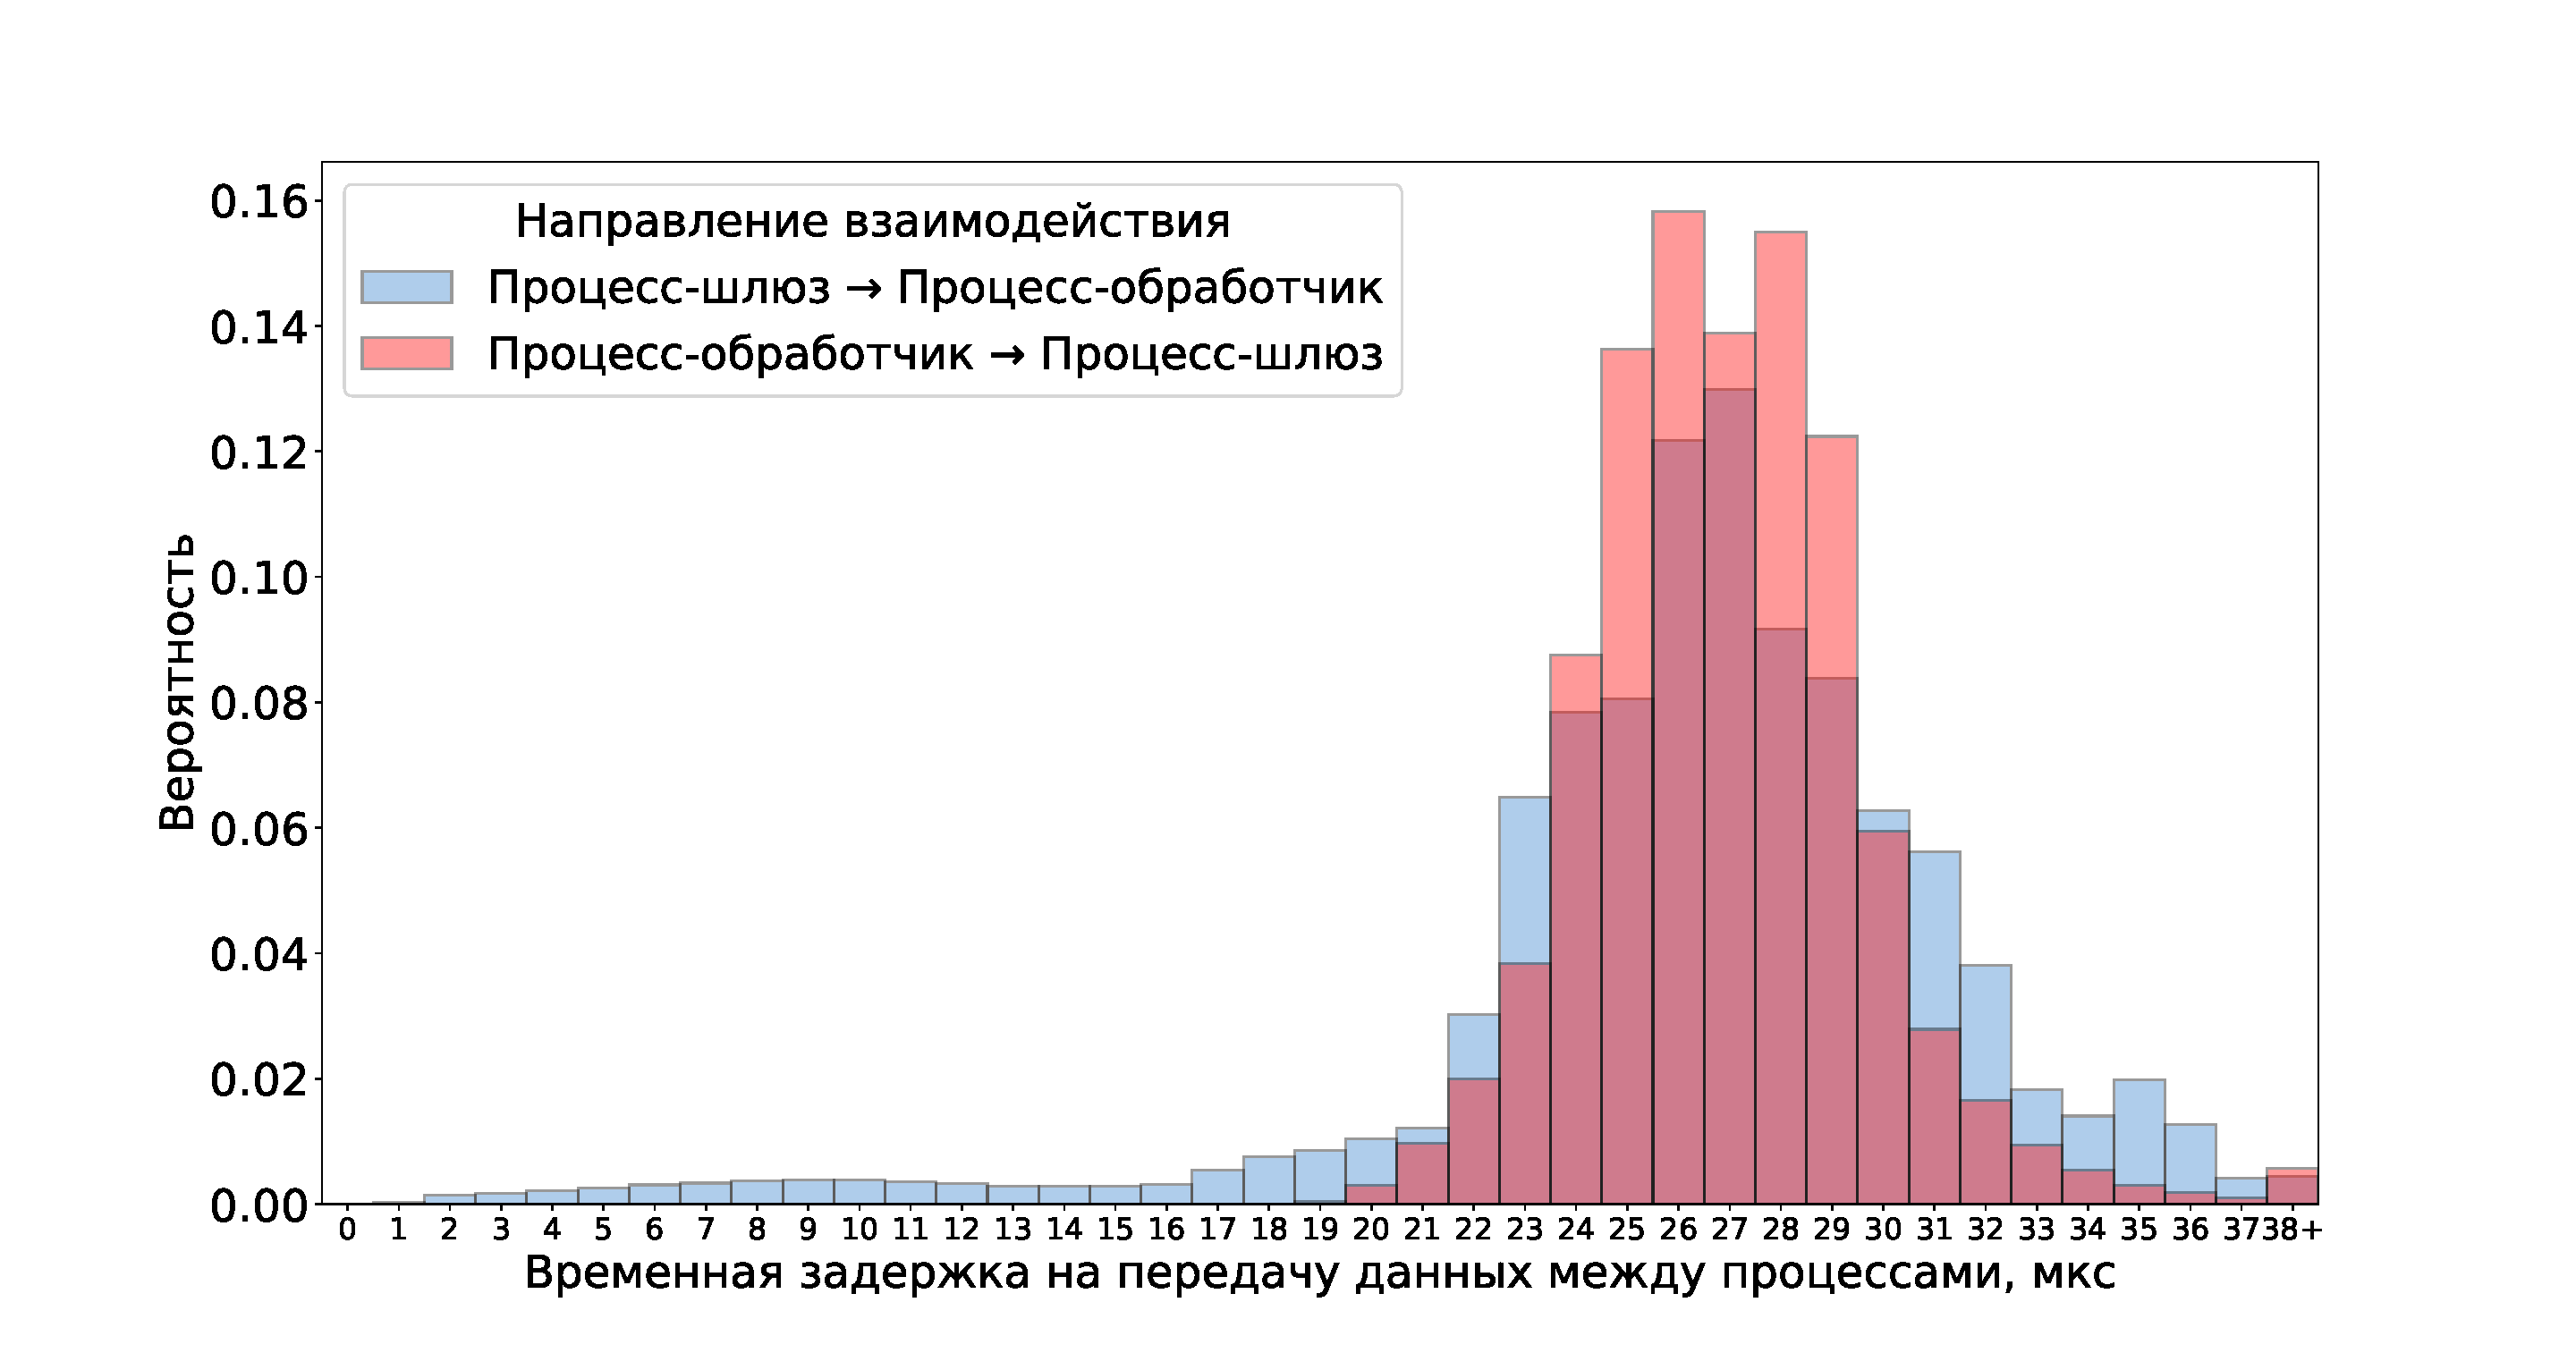
\includegraphics[width=\textwidth]{../../graphics/hist/SignalTCP}
\end{figure}

\begin{table}[!h]
\caption{Основные показатели временной задержки на передачу данных для метода, использующего разделяемую памяти для передачи данных и TCP для оповещения о появлении данных в ней}\label{chapter41:TableSignalTCP}
\centering
\begin{tabular}{|l|c|c|}
\hline
\begin{tabular}[c]{@{}l@{}}Направление\\ взаимодействия/\\ Показатель\end{tabular} & \multicolumn{1}{l|}{\begin{tabular}[c]{@{}l@{}}Процесс-шлюз $\rightarrow$\\ Процесс-обработчик\end{tabular}} & \multicolumn{1}{l|}{\begin{tabular}[c]{@{}l@{}}Процесс-обработчик $\rightarrow$\\ Процесс-шлюз\end{tabular}} \\ \hline
min(t), мкс & 1 & 3 \\ \hline
M(t), мкс & 22.5 $\pm$ 12.5 & 27.5 $\pm$ 5.5 \\ \hline
max(t), мс & 3 & 9.8 \\ \hline
\begin{tabular}[c]{@{}l@{}}$\Delta$, мс\end{tabular} & 10 $\pm$ 4 & 10 $\pm$ 4 \\ \hline
\begin{tabular}[c]{@{}l@{}}$\delta$, мкс\end{tabular} & 50 $\pm$ 27 & 87 $\pm$ 32 \\ \hline
\end{tabular}
\end{table}

В Таблице \ref{chapter41:TableSignalTCP} приведены основные временные характеристики данного метода. На Рисунке \ref{chapter41:FigSignalTCP} приведена гистограмма временной задержки на передачу данных для данного метода.

Как описано выше, значительная часть обслуживания заявки процессом-обработчиком происходит непосредственно в транспортном потоке. Из-за этого к моменту конца обработки текущей заявки очередная заявка уже может находиться в очереди в разделяемой памяти, что позволяет использовать оптимизацию, описанную в Разделе \ref{chapter31:SharedMemoryOptimization}. А именно принять и начать обслуживание очередной заявки, не используя дорогостоящий механизм оповещения, если заявка уже находится в очереди в разделяемой памяти. 

Прием заявки процессом-шлюзом не связан с обслуживанием заявки, поэтому к моменту, когда процесс-шлюз заканчивает прием и диспетчеризацию заявки, очередь входящих заявок в данном эксперименте пуста и поток-шлюз переходит к пассивному ожиданию новых заявок. Таким образом, приему и обслуживанию большинства заявок сопутствует пассивное ожидание сигнала по TCP, что негативно сказывается на временной задержке на передачу данных.

\subsection{Использование мультиплексора в разделяемой памяти для оповещения о появлении данных}

В данном подразделе приведены данные об экспериментах с семейством методов межпроцессного взаимодействия, описанными в Разделе \ref{chapter31:Mux}.

\subsubsection{Блокирующие методы}

В блокирующих методах поток мультиплексора событий использует примитив \textit{futex} 
\textbf{TBD:Может, сослаться на определение futex?}
для пассивного ожидания новых сигналов (см. Разделы \ref{chapter31:BlockingHSHA} и \ref{chapter31:BlockingLF}).

\paragraph{Диспетчеризация и обработка соединений по модели "Полусинхронный/Полуреактивный"}

Показатели потока исходящих заявок из симулятора в данном эксперименте: $\Delta \in$ \textit{10 $\pm$ 4 мс}, $\delta \in$ \textit{51 $\pm$ 28 мкс}.

В данном подразделе приведены данные об экспериментах с методом межпроцессного взаимодействия, описанным в Разделе \ref{chapter31:BlockingHSHA}.

\begin{figure}[!h]
\caption{Гистограмма временной задержки на передачу данных между процессами для метода, использующего разделяемую память для передачи данных, блокирующий мультиплексор в разделяемой памяти и метод ''Полусинхронный/Полуреактивный`` при обслуживании заявок}
\label{chapter41:FigBlockingHSHA}
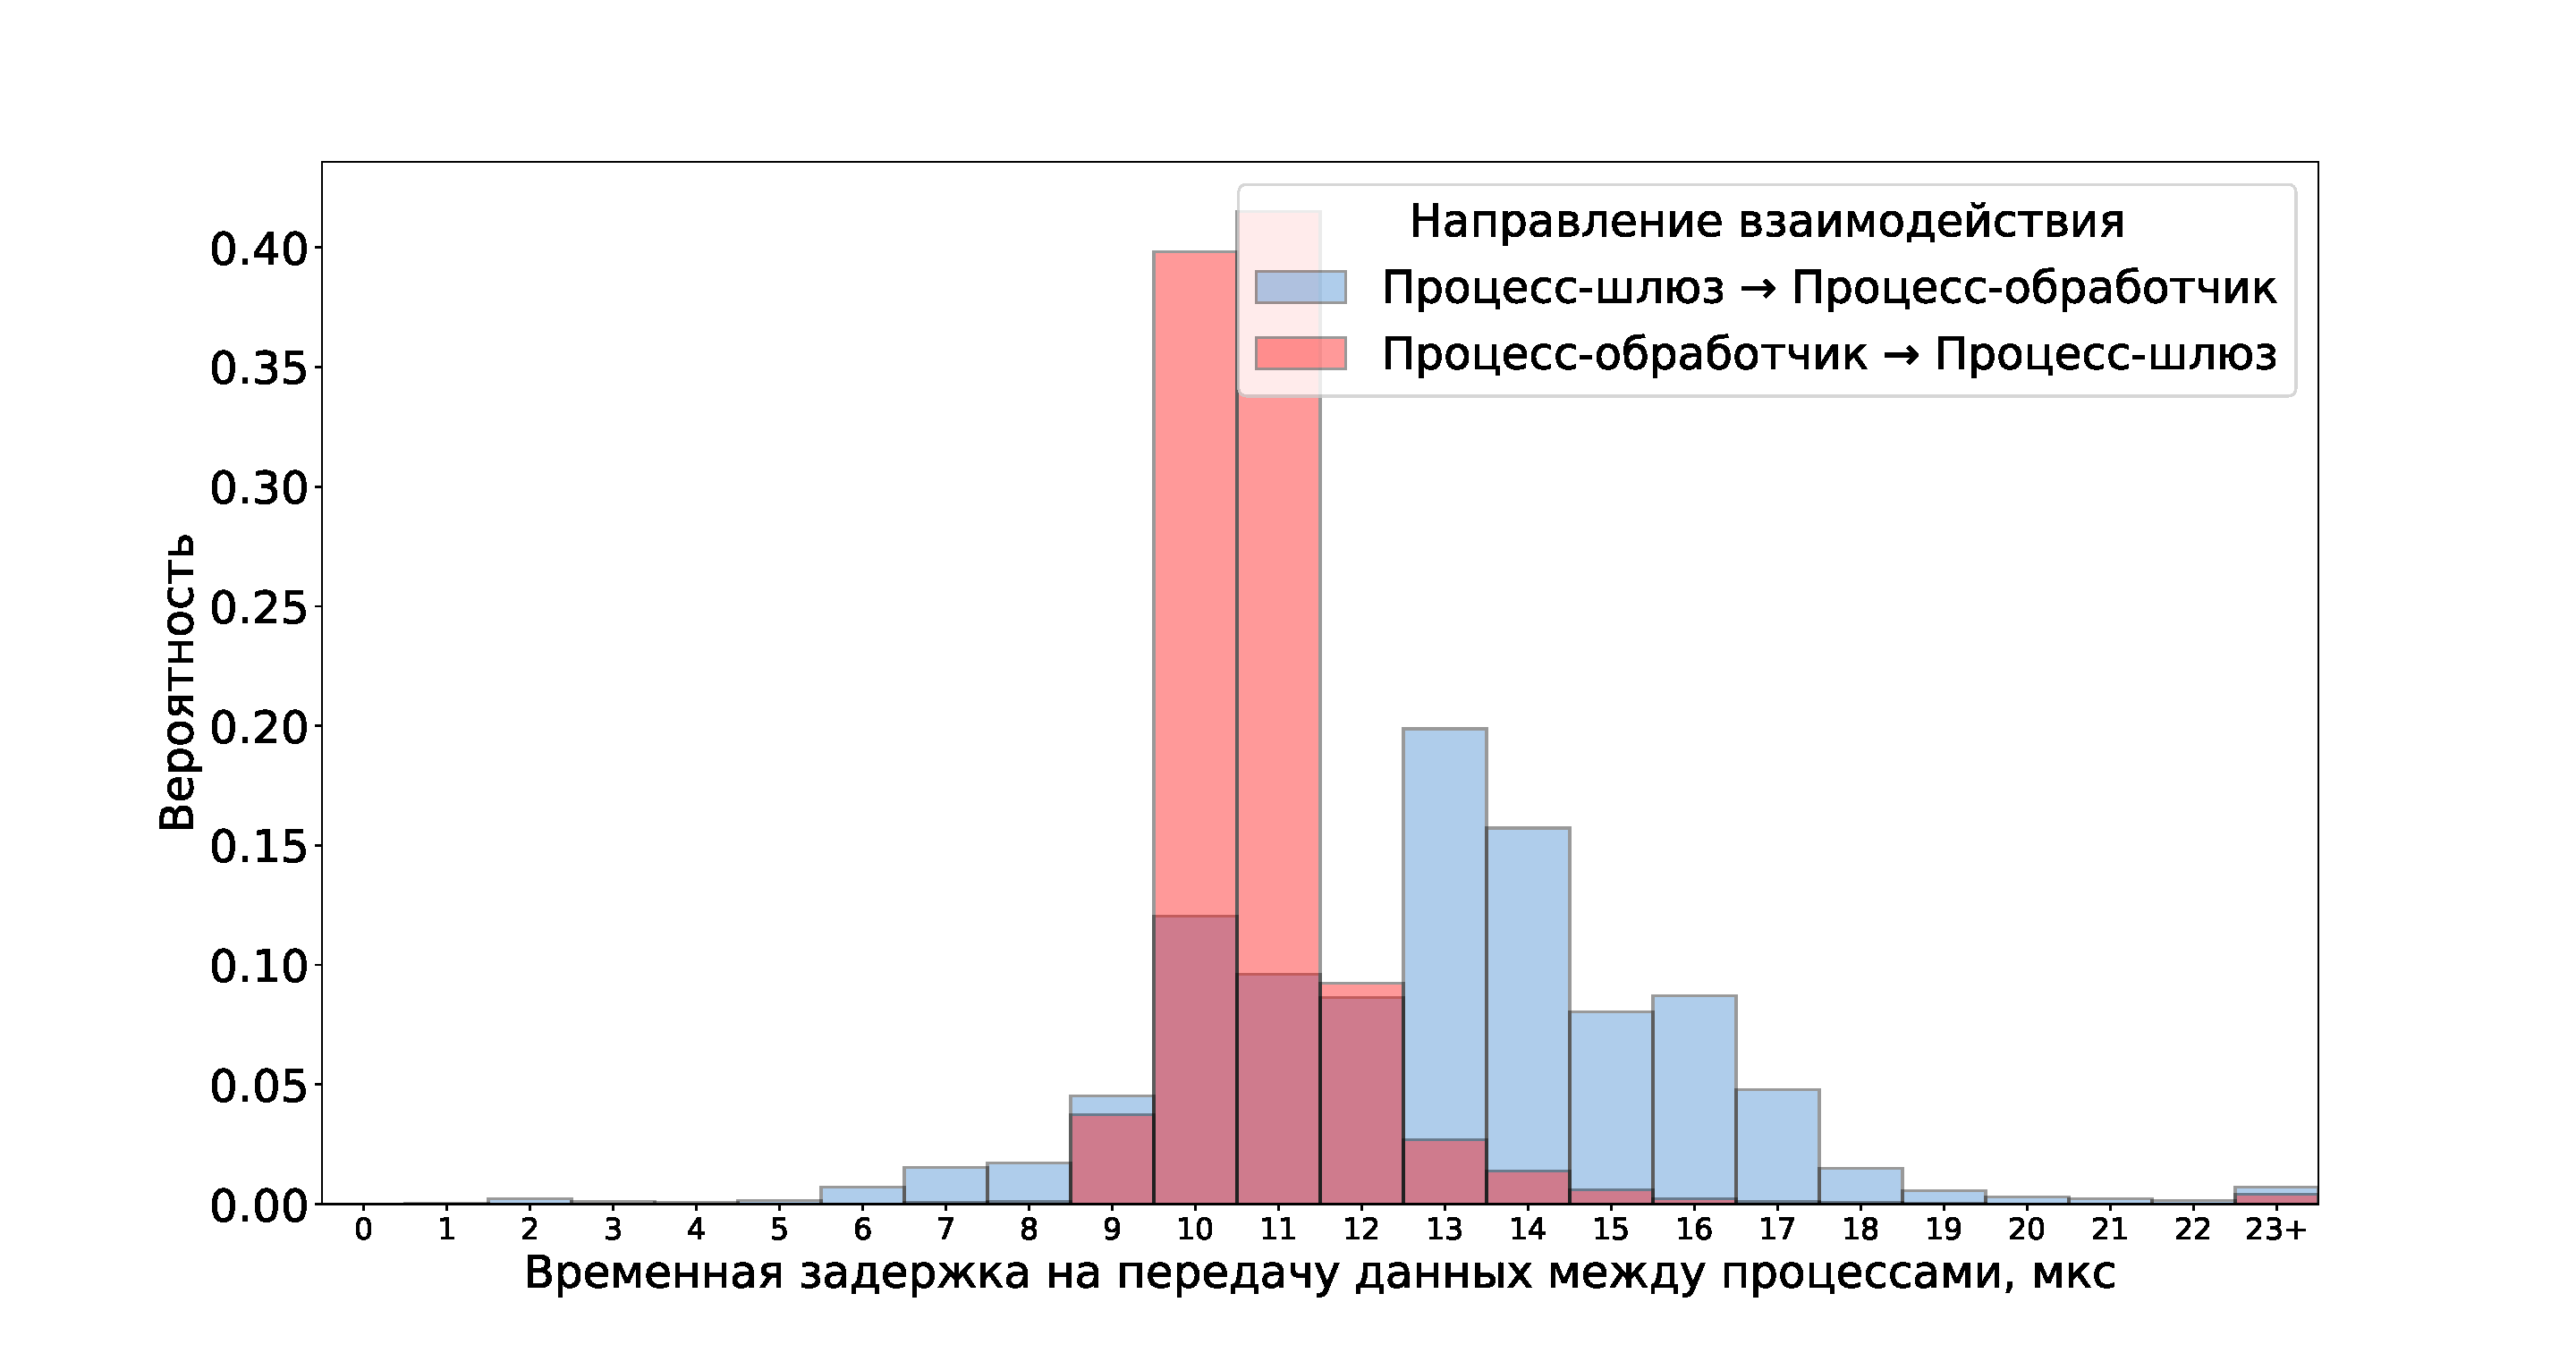
\includegraphics[width=\textwidth]{../../graphics/hist/BlockingHSHA}
\end{figure}

\begin{table}[!h]
\caption{Основные показатели временной задержки на передачу данных между процессами для метода, использующего разделяемую память для передачи данных, блокирующий мультиплексор в разделяемой памяти и метод ''Полусинхронный/Полуреактивный`` при обслуживании заявок}\label{chapter41:TableBlockingHSHA}
\centering
\begin{tabular}{|l|c|c|}
\hline
\begin{tabular}[c]{@{}l@{}}Направление\\ взаимодействия/\\ Показатель\end{tabular} & \multicolumn{1}{l|}{\begin{tabular}[c]{@{}l@{}}Процесс-шлюз $\rightarrow$\\ Процесс-обработчик\end{tabular}} & \multicolumn{1}{l|}{\begin{tabular}[c]{@{}l@{}}Процесс-обработчик $\rightarrow$\\ Процесс-шлюз\end{tabular}} \\ \hline
min(t), мкс & 1 & 3 \\ \hline
M(t) $\pm$ 95\%, мкс & 12.5 $\pm$ 5.5 & 11.5 $\pm$ 2.5 \\ \hline
max(t), мс & 6.9 & 11.6 \\ \hline
\begin{tabular}[c]{@{}l@{}}$\Delta$, мс\end{tabular} & 10 $\pm$ 4 & 10 $\pm$ 4 \\ \hline
\begin{tabular}[c]{@{}l@{}}$\delta$, мкс\end{tabular} & 51 $\pm$ 28 & 91 $\pm$ 36 \\ \hline
\end{tabular}
\end{table}

В Таблице \ref{chapter41:TableBlockingHSHA} приведены основные временные характеристики данного метода. На Рисунке \ref{chapter41:FigBlockingHSHA} приведена гистограмма временной задержки на передачу данных для данного метода.

Использовании более эффективного метода межпроцессного взаимодействия наглядно показывает эффект от влияния времени обслуживания заявки в транспортном потоке на временную задержку на передачу данных. Процесс-шлюз с минимальной временной задержкой принимает и диспетчеризует заявку для дальнейшей обработки и сразу же готов принимать следующую заявку. Процесс-обработчик же использует транспортный поток для частичного обслуживания заявки (см. Рисунок \ref{chapter41:EngineLatency}), а потому в среднем временная задержка на передачу данных имеет худшие показатели, так как это может задерживать прием очередных заявок.

\paragraph{Диспетчеризация и обработка соединений по модели "Лидер/Последователи"}

Показатели потока исходящих заявок из симулятора в данном эксперименте: $\Delta \in$ \textit{8.4 $\pm$ 5.3 мс}, $\delta \in$ \textit{52 $\pm$ 28 мкс}.

В данном подразделе приведены данные об экспериментах с методом межпроцессного взаимодействия, описанным в Разделе \ref{chapter31:BlockingLF}.

В Таблице \ref{chapter41:TableBlockingLF} приведены основные временные характеристики данного метода. \textbf{TBD}

На Рисунке \ref{chapter41:FigBlockingLF} приведена гистограмма временной задержки на передачу данных для данного метода.

\begin{figure}[!h]
\caption{Гистограмма временной задержки на передачу данных между процессами для метода, использующего разделяемую память для передачи данных, блокирующий мультиплексор в разделяемой памяти и метод ''Лидер/Последователи`` при обслуживании заявок}
\label{chapter41:FigBlockingLF}
\includegraphics[width=\textwidth]{../../graphics/hist/BlockingLF}
\end{figure}

\begin{table}[!h]
\caption{Основные показатели временной задержки на передачу данных между процессами для метода, использующего разделяемую память для передачи данных, блокирующий мультиплексор в разделяемой памяти и метод ''Лидер/Последователи`` при обслуживании заявок}\label{chapter41:TableBlockingLF}
\centering
\begin{tabular}{|l|c|c|}
\hline
\begin{tabular}[c]{@{}l@{}}Направление\\ взаимодействия/\\ Показатель\end{tabular} & \multicolumn{1}{l|}{\begin{tabular}[c]{@{}l@{}}Процесс-шлюз $\rightarrow$\\ Процесс-обработчик\end{tabular}} & \multicolumn{1}{l|}{\begin{tabular}[c]{@{}l@{}}Процесс-обработчик $\rightarrow$\\ Процесс-шлюз\end{tabular}} \\ \hline
min(t), мкс & 1 & 2 \\ \hline
M(t) $\pm$ 95\%, мкс & 11.5 $\pm$ 6.5 & 9.5 $\pm$ 1.5 \\ \hline
max(t), мс & 2.4 & 9.5 \\ \hline
\begin{tabular}[c]{@{}l@{}}$\Delta$, мс\end{tabular} & 8.4 $\pm$ 5.3 & 8.4 $\pm$ 5.3 \\ \hline
\begin{tabular}[c]{@{}l@{}}$\delta$, мкс\end{tabular} & 52 $\pm$ 29 & 90 $\pm$ 35 \\ \hline
\end{tabular}
\end{table}

Аналогичный эффект как при использовании предыдущего метода наблюдается и при использовании метода ''Лидер/Последователи``. Отличие состоит в меньшей временной задержке на передачу данных в пределах 1-2 мкс.

\subsubsection{Неблокирующий метод}

В неблокирующем методе поток мультиплексора событий метод активного ожидания новых сигналов (см. Раздел \ref{chapter31:NonBlockingLF}). В данном параграфе рассматривается исключительно метод обслуживания заявок ''Лидер/Последователи`` т.к. в параграфе выше она показала лучший результат по сравнению с методом обслуживания заявок ''Полусинхронный/Полуреактивный``.

\paragraph{Диспетчеризация и обработка соединений по модели "Лидер/Последователи"}

Показатели потока исходящих заявок из симулятора в данном эксперименте: $\Delta \in$ \textit{7.1 $\pm$ 5.8 мс}, $\delta \in$ \textit{83 $\pm$ 61 мкс}.

В данном подразделе приведены данные об экспериментах с методом межпроцессного взаимодействия, описанным в Разделе \ref{chapter31:NonBlockingLF}.

В Таблице \ref{chapter41:TableNonBlockingLF} приведены основные временные характеристики данного метода. На Рисунке \ref{chapter41:FigNonBlockingLF} приведена гистограмма временной задержки на передачу данных для данного метода.

\begin{figure}[!h]
\caption{Гистограмма временной задержки на передачу данных между процессами для метода, использующего разделяемую память для передачи данных, неблокирующий мультиплексор в разделяемой памяти и модель ''Лидер/Последователи`` при обслуживании заявок}
\label{chapter41:FigNonBlockingLF}
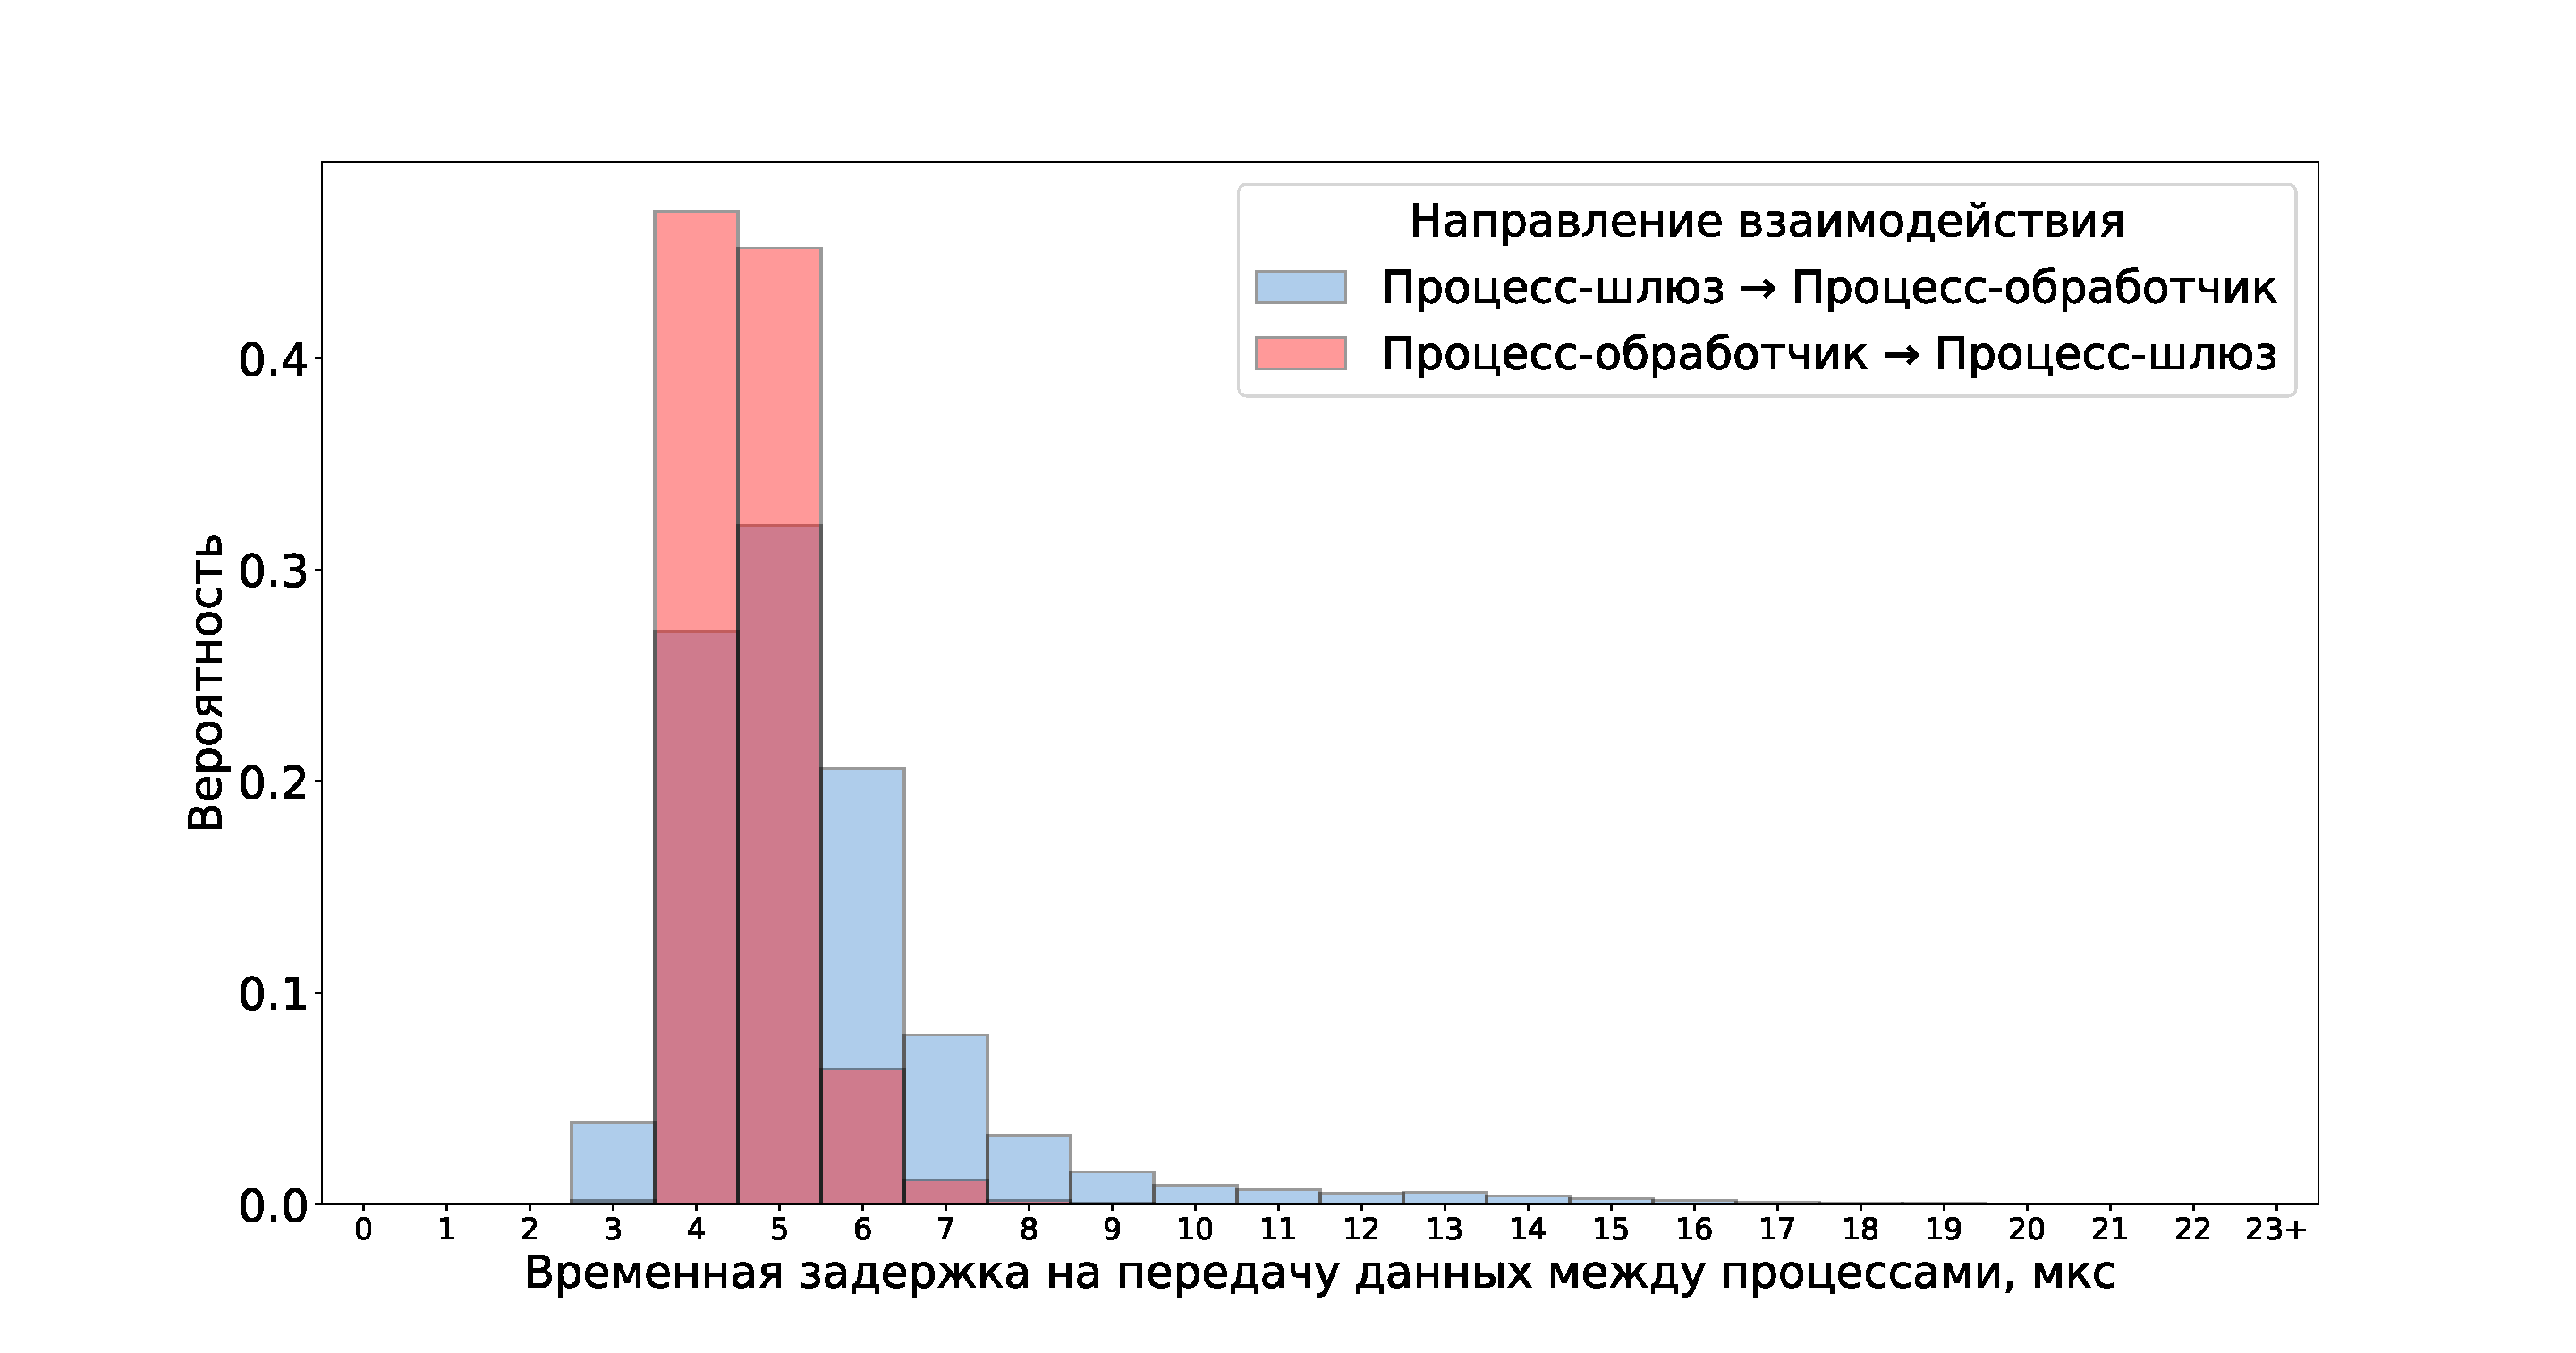
\includegraphics[width=\textwidth]{../../graphics/hist/NonBlockingLF}
\end{figure}

\begin{table}[!h]
\caption{Основные показатели временной задержки на передачу данных между процессами для метода, использующего разделяемую память для передачи данных, неблокирующий мультиплексор в разделяемой памяти и модель ''Лидер/Последователи`` при обслуживании заявок}\label{chapter41:TableNonBlockingLF}
\centering
\begin{tabular}{|l|c|c|}
\hline
\begin{tabular}[c]{@{}l@{}}Направление\\ взаимодействия/\\ Показатель\end{tabular} & \multicolumn{1}{l|}{\begin{tabular}[c]{@{}l@{}}Процесс-шлюз $\rightarrow$\\ Процесс-обработчик\end{tabular}} & \multicolumn{1}{l|}{\begin{tabular}[c]{@{}l@{}}Процесс-обработчик $\rightarrow$\\ Процесс-шлюз\end{tabular}} \\ \hline
min(t), мкс & 1 & 3 \\ \hline
M(t) $\pm$ 95\%, мкс & 6 $\pm$ 2 & 5 $\pm$ 1 \\ \hline
max(t), мс & 0.064 & 0.017 \\ \hline
\begin{tabular}[c]{@{}l@{}}$\Delta$, мс\end{tabular} & 7.1 $\pm$ 5.8 & 7.1 $\pm$ 5.8 \\ \hline
\begin{tabular}[c]{@{}l@{}}$\delta$, мкс\end{tabular} & 220 $\pm$ 197 & 326 $\pm$ 272 \\ \hline
\end{tabular}
\end{table}

Метод с активным ожиданием событий на мультиплексоре в разделяемой памяти ожидаемо показывает лучший результат по сравнению со всеми ранее рассмотренными методами. Это происходит потому что в данном случае нет необходимости пробуждать и дожидаться пробуждения потока для обслуживания заявки. Исходя из разницы временной задержки на передачу данных в неблокирующем и блокирующим методах, пробуждение потока до постановки его на выполнение занимает около 5-6 мкс.
\textbf{TBD: а надо ли оно мне? Вопрос корректности приведения циклов на AMD к секундам спорный}
В работе другого автора \cite{8526899} была измерена временная задержка на пробуждение потоков, прикрепленных к разным ядрам разных процессоров, посредством системного вызова futex. Измерения проводились на процессоре AMD Opteron 6272 и показали $\mu = 24640.5$ машинных циклов от системного вызова до выполнения первой инструкции пробужденным потоком. Или $\frac{24640.5~\text{машинных~циклов}}{2.1~*~10^9~\text{Гц}} \approx 11 ~\text{мкс}$ при частоте процессора 2.1 ГГц, что похоже на обозначенный выше результат с учетом использования в настоящей работе более современного аппаратного обеспечения.

Для данного метода распределение временной задержки на передачу данных от процесса-обработчика к процессу-шлюзу схоже с предыдущими методами, но этот показатель существенно отличается при передаче от процесса-шлюза к процессу-обработчику. Это может быть вызвано тем, что более быстрый метод межпроцессного взаимодействия при данной постановке эксперимента приводит к отсутствию и, как следствие, время обслуживания заявки в транспортном потоке процесса-обработчика не влияет на временную задержку на передачу данных.

Данный подход обладает существенным \textbf{недостатком}. Поскольку поток, активно опрашивающий мультиплексор, исполняется до получения и обработки события, то существует возможность, что планировщик ОС вытеснит этот поток с процессора. Стандартный квант планирования потоков в Linux -- 100 мс. Если событие не будет получено и обработано за это время, то поток может быть вытеснен с процессора и временная задержка на передачу данных увеличится на сотни миллисекунд. Данный недостаток не проявляется в проведенном эксперименте, поскольку что интервал $\Delta$ между сериями заявок значительно меньше 100 мс.

\textbf{TBD: объяснить разброс в интервалах между заявками.}


\chapterconclusion

Проведено экспериментальное сравнение разработанных методов межпроцессного взаимодействия.
\begin{enumerate}
\item Методы межпроцессного взаимодействия, использующие мультиплексор в разделяемой памяти для оповещения о появлении данных в очереди в разделяемой памяти имеют существенно меньшую временную задержку на передачу данных, чем метод, использующий для этого TCP. А именно, \textit{17 мкс} и \textit{10 мкс} для 95 процентиля для пассивного варианта ''Лидер/Последователи`` против \textit{34 мкс} и \textit{31 мкс} для 95 процентиля для TCP с передачей данных через очередь в разделяемой памяти.
\item В семействе пассивных методов межпроцессного взаимодействия на основе мультиплексора в разделяемой памяти наименьшую временную задержку на передачу данных показала вариация с использованием метода обслуживания заявок ''Лидер/Последователи``, а именно \textit{17 мкс} и \textit{10 мкс} для 95 процентиля против \textit{17 мкс} и \textit{13 мкс} для 95 процентиля при использовании метода обслуживания заявок ''Полусинхронный/Полуреактивный``.
\item Самой низкой временной задержки на передачу данных удалось добиться при использовании активно опрашивающей мультиплексор вариации метода межпроцессного взаимодействия, использующего метод ''Лидер/Последователи`` при обслуживании заявок. А именно, \textit{7 мкс} и \textit{6 мкс} для 95 процентиля.
\item При использовании пассивных методов на основе мультиплексора в разделяемой памяти заметны эффекты от обслуживания заявок в транспортном потоке на временную задержку на передачу данных. В проведенном эксперименте в процессе-шлюзе заявки частично обслуживаются именно в транспортном потоке, из-за чего могут образовываться очереди и увеличиваться временная задержка на передачу данных. В активно опрашивающем методе этот эффект не заметен, так как временная задержка на передачу данных меньше, соответственно, меньше временная задержка реакции на очередную заявку и, следовательно, меньше возможностей для формирования очереди из заявок.
\item Активно опрашивающий мультиплексор метод обладает существенным недостатком. поток, активно опрашивающий мультиплексор в разделяемой памяти, может быть вытеснен с процессора по окончании отведенного ему кванта процессорного времени -- 100 миллисекунд. В проведенном эксперименте данный эффект не наблюдается, так как серии заявок отправляются симулятором в систему на порядок чаще, с интервалом примерно 10 миллисекунд. Данный недостаток может быть необходимо разрешить для обеспечения должного уровня качества обслуживания заявок в системе.
\end{enumerate}

%% Макрос для заключения. Совместим со старым стилевиком.
\startconclusionpage

Целью настоящей работы являлось уменьшение временной задержки на передачу данных между процессами в пределах одного физического узла путем разработки и применения методов эффективного межпроцессного взаимодействия. Было выполнено сравнение методов межпроцессного взаимодействия и синхронизации. Исследованы подходы других авторов. Разработаны и реализованы новые методы межпроцессного взаимодействия. Проведено экспериментальное исследование разработанных методов межпроцессного взаимодействия.

Результатом работы стало семейство новых методов межпроцессного взаимодействия. Передача данных в них осуществляется через очередь в разделяемой памяти. Оповещение о появлении данных в очереди осуществляется через разработанный и реализованный мультиплексор оповещений в разделяемой памяти. Он позволяет производить большую часть операций по оповещению процесса-читателя в пользовательской памяти, а ядро использовать только при необходимости процессу-читателю ожидать оповещений в режиме сна и процессу-писателю разбудить его.

Были реализованы различные методы обслуживания соединений по полученным из мультиплексора оповещениям, исследовано влияние активного опроса мультиплексора на временную задержку на передачу данных. Исходя из полученных результатов, разработанные в данной работе методы показали существенно меньшую временную задержку на передачу данных по сравнению с методами, использующими TCP. Метод обслуживания соединений ''Лидер/Последователи`` при использовании с мультиплексором оповещений в разделяемой памяти показывает  меньшую временную задержку на передачу данных, чем метод обслуживания соединений ''Полусинхронный/Полуреактивный``. Применение метода активного опроса мультиплексора позволило существенно уменьшить временную задержку на передачу данных по сравнению с аналогичным методом с пассивным ожиданием оповещений в режиме сна.

Основные результаты работы представлены на IX Конгрессе Молодых Ученых. Результаты работы использованы в программной платформе для высокочастотной алгоритмической торговли Tbricks компании Itiviti.

\printmainbibliography

%% После этой команды chapter будет генерировать приложения, нумерованные русскими буквами.
%% \startappendices из старого стилевика будет делать то же самое
\appendix

\chapter{Исходный код алгоритмов работы с мультиплексором событий в разделяемой памяти}\label{sec:app:1}

\begin{algorithm}[!h]
\caption{Исходный код процедуры получения оповещений из мультиплексора событий в разделяемой памяти}
\label{appendix91:ReceiverCode}
\begin{lstlisting}[frame=tlrb]
void MutliplexerServer::handle_signals() {
	// Шаг 1. Если в futex записан 0, значит, нет оповещений для обработки. Тогда процесс переходит в состояние сна.
	m_mux->wait();
	// Шаг 2. Атомарно получить актуальное значение futex и установить вместо него 0.
	int32_t futex = atomic_exchange(&m_futex, 0);
	// Шаг 3. Подсчитать количество установленных битов в числе, чтобы не выполнять линейное сканирование всех 32 битов.
	uint8_t cnt = popcnt(futex);
	for (uint8_t i = 0; i < cnt; i++) {
		// Шаг 4. Для каждого бита futex проверить соответствующие ему сигнальные числа.
		uint8_t f = get_unset_lsb(&futex);
		// Шаг 5. Атомарно получить значение сигнального числа и записать в него 0.
		int64_t signal = atomic_exchange(&m_signal[f], 0);
		uint8_t nsignals = popcntl(signal);
		// Шаг 6. Для каждого найденного сигнала запустить его обработку.
		for (uint8_t j = 0; j < nsignals; j++) {
			uint8_t s = get_unset_lsb(&signal);
			this->handle_signal(i * 64 + s);
		}
	}
}

// Ожидание новых оповещений на futex в режиме сна или методом активного опроса мультиплексора.
void Multiplexer::wait();
// Выполняет обработку соединения, которому ранее был выдан номер id
void MultiplexerServer::handle_signal(Signal id);

// Возвращает количество выставленных битов в числе
uint8_t popcnt(int32_t value);
uint8_t popcntl(int64_t value);

// Сбрасывает младший бит числа и возвращает позицию этого бита.
uint8_t get_unset_lsb(uint32_t & value);
uint8_t get_unset_lsb(uint64_t & value);
\end{lstlisting}
\end{algorithm}

\begin{algorithm}[!h]
\caption{Исходный код процедуры получения оповещений из мультиплексора событий в разделяемой памяти для метода обслуживания соединений ''Лидер/Последователи``}
\label{appendix91:LFReceiverCode}
\begin{lstlisting}[frame=tlrb]
void MutliplexerServer::handle_signals() {
	// Шаг 1. Если в futex записан 0, значит, нет оповещений для обработки. Тогда процесс переходит в состояние сна.
	m_mux->wait();
	int32_t futex = atomic_exchange(&m_futex, 0);
	std::vector<int32_t> signals;
	listeners.reserve(Multiplexer::c_signals_per_mux);
	uint8_t cnt = popcnt(futex);
	for (uint8_t i = 0; i < cnt; i++) {
		uint8_t f = get_unset_lsb(&futex);
		int64_t signal = atomic_exchange(&m_signal[f], 0);
		uint8_t nsignals = popcntl(signal);
		// Шаг 6. Для каждого найденного сигнала запустить его обработку.
		for (uint8_t j = 0; j < nsignals; j++) {
			uint8_t s = get_unset_lsb(&signal);
			// Для каждого полученного оповещения
			// отметить соединение как Handling,
			// либо проигнорировать оповещение
			if (this->should_handle(i * 64 + s)) {
				signals.emplace_back(i * 64 + s);
			}
		}
	}
	
	// Создать нового лидера, который будет
	// выполнять процедуру handle_signals следующим
	m_thread_pool->promote_new_leader();
	
	// Непосредственно обслуживание соединений по полученным оповещениям
	for (int32_t signal : signals) {
		this->handle_signal(i * 64 + s);
	}
}

// Возвращает true, если соединение было Idle, и помечает его Handling
// Если соединение в состоянии Handling, то переводит его в состояние KeepHandling
// Возвращает false, если любое другое состояние.
bool MultiplexerServer::should_handle(Signal id);
\end{lstlisting}
\end{algorithm}

%
%В приложениях рисунки, таблицы и другие подобные элементы нумеруются по приложениям с соответствующим префиксом. Проверим это.
%
%листинг~\ref{lst4:apx} должен иметь номер А.1.
%
%\begin{algorithm}[!h]
%\caption{Исходный код и флоат \texttt{algorithm}}\label{lst4:apx}
%\begin{lstlisting}
%public class HelloWorld {
%    public static void main(String[] args) {
%        System.out.println("Hello, world!");
%    }
%}
%\end{lstlisting}
%\end{algorithm}
%
%рисунок~\ref{fig2:apx} должен иметь номер A.1.
%
%\begin{figure}[!h]
%\caption{Пример рисунка}\label{fig2:apx}
%\centering
%\begin{tikzpicture}[scale=0.7]
%\draw[thick,->] (0,0)--(3.5,0);
%\draw[thick,->] (0,0)--(0,3.5);
%\draw[very thick, red] (0,0)--(3,3);
%\draw[dashed] (3,0)--(3,3);
%\draw[dashed] (1.5,0)--(1.5,1.5);
%\end{tikzpicture}
%\end{figure}
%
%таблица~\ref{tab3:apx} должна иметь номер A.1.
%
%\begin{table}[!h]
%\caption{таблица умножения с помощью \texttt{tabularx} (фрагмент)}\label{tab3:apx}
%\centering
%\begin{tabularx}{\textwidth}{|*{18}{>{\centering\arraybackslash}X|}}\hline
%-- & 1 & 2 & 3 & 4 & 5 & 6 & 7 & 8 & 9 & 10 & 11 & 12 & 13 & 14 & 15 & 16 & 17 \\\hline
%1  & 1 & 2 & 3 & 4 & 5 & 6 & 7 & 8 & 9 & 10 & 11 & 12 & 13 & 14 & 15 & 16 & 17 \\\hline
%2  & 2 & 4 & 6 & 8 & 10 & 12 & 14 & 16 & 18 & 20 & 22 & 24 & 26 & 28 & 30 & 32 & 34 \\\hline
%3  & 3 & 6 & 9 & 12 & 15 & 18 & 21 & 24 & 27 & 30 & 33 & 36 & 39 & 42 & 45 & 48 & 51 \\\hline
%4  & 4 & 8 & 12 & 16 & 20 & 24 & 28 & 32 & 36 & элементов40 & 44 & 48 & 52 & 56 & 60 & 64 & 68 \\\hline
%\end{tabularx}
%\end{table}
%
%Заодно проверим нумерованные и ненумерованные перечисления. Ненумерованные:
%\begin{itemize}
%    \item пункт А;
%    \item пункт Б;
%    \item пункт В.
%\end{itemize}
%
%Нумерованные списки нескольких уровней:
%\begin{enumerate}
%    \item первый элемент;
%    \item второй элемент с подэлементами:
%    \begin{enumerate}
%        \item первый подэлемент;
%        \item второй подэлемент;
%        \item третий подэлемент.
%    \end{enumerate}
%    \item третий элемент;
%    \item четвертый элемент;
%    \item пятый элемент;
%    \item шестой элемент;
%    \item седьмой элемент;
%    \item восьмой элемент;
%    \item девятый элемент;
%    \item десятый элемент.
%\end{enumerate}
%
%\chapter{Еще один пример приложения с неимоверно длиннющим названием для тестирования переносов}\label{sec:app:2}
%
%Проверим на примере таблиц, что нумерация в приложениях~--- по приложениям.
%таблица~\ref{tab3:apx2} должна иметь номер Б.1.
%
%\begin{table}[!h]
%\caption{таблица умножения с помощью \texttt{tabularx} (фрагмент)}\label{tab3:apx2}
%\centering
%\begin{tabularx}{\textwidth}{|*{18}{>{\centering\arraybackslash}X|}}\hline
%-- & 1 & 2 & 3 & 4 & 5 & 6 & 7 & 8 & 9 & 10 & 11 & 12 & 13 & 14 & 15 & 16 & 17 \\\hline
%1  & 1 & 2 & 3 & 4 & 5 & 6 & 7 & 8 & 9 & 10 & 11 & 12 & 13 & 14 & 15 & 16 & 17 \\\hline
%2  & 2 & 4 & 6 & 8 & 10 & 12 & 14 & 16 & 18 & 20 & 22 & 24 & 26 & 28 & 30 & 32 & 34 \\\hline
%3  & 3 & 6 & 9 & 12 & 15 & 18 & 21 & 24 & 27 & 30 & 33 & 36 & 39 & 42 & 45 & 48 & 51 \\\hline
%4  & 4 & 8 & 12 & 16 & 20 & 24 & 28 & 32 & 36 & 40 & 44 & 48 & 52 & 56 & 60 & 64 & 68 \\\hline
%\end{tabularx}
%\end{table}
%
%\chapter{Пример огромного листинга}
%
%\begin{lstlisting}[caption={Пример большого листинга},label={lstX}]
%import java.util.*;
%
%public class Example {
%    static int[] restoreOutgoing(int[] g, int[] outgoing,
%                                 int vertex, int mask) {
%        int[] rv = new int[1 + Integer.bitCount(mask)];
%        int n = g.length;
%        int current = rv.length - 1;
%        while (true) {
%            rv[current] = vertex;
%            if (current == 0) {
%                if (vertex != 0) {
%                    throw new AssertionError();
%                }
%                return rv;
%            }
%            mask ^= 1 << (vertex - 1);
%            int prevMask = outgoing[mask] & g[vertex];
%            if (prevMask == 0) {
%                throw new AssertionError();
%            }
%            vertex = Integer.numberOfTrailingZeros(prevMask);
%            --current;
%        }
%    }
%
%    static int[] restoreIncoming(int[] g, int[] incoming,
%                                 int vertex, int mask) {
%        int[] rv = new int[1 + Integer.bitCount(mask)];
%        int n = g.length;
%        int current = 0;
%        while (true) {
%            rv[current] = vertex;
%            if (current == rv.length - 1) {
%                if (vertex != 0) {
%                    throw new AssertionError();
%                }
%                return rv;
%            }
%            mask ^= 1 << (vertex - 1);
%            int nextMask = incoming[mask] & g[vertex];
%            if (nextMask == 0) {
%                throw new AssertionError();
%            }
%            vertex = Integer.numberOfTrailingZeros(nextMask);
%            ++current;
%        }
%    }
%}
%\end{lstlisting}
%                

\end{document}